\label{2.5 C8M Answer Key}
\subsection{Answer Key}
\tiny
\renewcommand{\insertclass}{- Class 8}
\renewcommand{\insertsubject}{ - Math}

\begin{frame}[shrink=0.1,label=QPC8QC5BM - BM - Q10]{Q1 [Basic Math]}
\vspace{-0.2cm}
\mcqtextbottomOneFour{
questionnumber={1}, 
questionTag={C5BM - BM - Q10}, 
questiontext={A farmer harvested 9 rows of potatoes, and each row had 15 potatoes. How many potatoes are there in the entire garden?},
optionA={24},
optionB={135},
optionC={6},
optionD={945},
correctoption={B},
}

\begin{minipage}{\linewidth}
\hspace{1cm}
\centering
\tiny
\renewcommand{\arraystretch}{1.25}
\begin{tabular}{|M{1.2cm}|M{0.8cm}|M{0.8cm}|M{0.8cm}|M{0.8cm}|M{0.8cm}|}
\hline
Option & A (\ding{55}) & \cellcolor{cellgreen} B (\ding{51}) & C (\ding{55}) & D (\ding{55}) & E \\ 
\hline
8 A & \highno{8\%} & \highgreen{85\%} & \highno{0\%} & \highno{0\%} & \highno{8\%} \\ 
 \hline 
8 B & \highno{0\%} & \highgreen{100\%} & \highno{0\%} & \highno{0\%} & \highno{0\%} \\ \hline
\end{tabular}
\end{minipage}

\end{frame}
% \input{4. PPT/6. My Answer/Math/C8/117_C8M - Q1}


\begin{frame}[shrink=0.1,label=QPC8QC6M02 - BM - Q2]{Q2 [Basic Math]}
\vspace{-0.2cm}
\mcqtextbottomOneFour{
questionnumber={2}, 
questionTag={C6M02 - BM - Q2}, 
questiontext={Solve using the BODMAS rule. \quad 12 $-$ 13 $\times$ 12 $+$ (15 $\divisionsymbol$ 3)},
optionA={$-$17},
optionB={160},
optionC={$-$139},
optionD={7},
correctoption={C},
}

\begin{minipage}{\linewidth}
\hspace{1cm}
\centering
\tiny
\renewcommand{\arraystretch}{1.25}
\begin{tabular}{|M{1.2cm}|M{0.8cm}|M{0.8cm}|M{0.8cm}|M{0.8cm}|M{0.8cm}|}
\hline
Option & A (\ding{55}) & B (\ding{55}) & \cellcolor{cellgreen} C (\ding{51}) & D (\ding{55}) & E \\ 
\hline
8 A & \highno{23\%} & \highno{23\%} & \highred{38\%} & \highno{8\%} & \highno{8\%} \\ 
 \hline 
8 B & \highno{7\%} & \highno{0\%} & \highgreen{87\%} & \highno{7\%} & \highno{0\%} \\ \hline
\end{tabular}
\end{minipage}

\end{frame}
\begin{frame}{Q2 - My Answer Responses}
    \vspace{-0.6cm}
    \begin{multicols}{3}

    % Image: Q2_D117220_Math.png - Scaled height: 5.05mm
    \begin{minipage}{\linewidth}
    \RaggedRight\textbf{\tiny \highred{Vipulan J R [A]}} \\ 
    \vspace{4.00pt}\fcolorbox{blue}{white}{
\includegraphics[width=3cm]{Q2_D117220_Math.png}}
    \end{minipage}
    \vspace{10pt}

    % Image: Q2_D117221_Math.png - Scaled height: 33.48mm
    \begin{minipage}{\linewidth}
    \RaggedRight\textbf{\tiny \highgreen{Dharani B [C]}} \\ 
    \vspace{4.00pt}\fcolorbox{blue}{white}{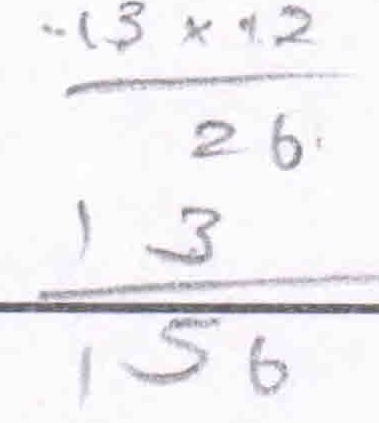
\includegraphics[width=3cm]{Q2_D117221_Math.png}}
    \end{minipage}
    \vspace{10pt}

    % Image: Q2_D117227_Math.png - Scaled height: 6.79mm
    \begin{minipage}{\linewidth}
    \RaggedRight\textbf{\tiny \highgreen{Subiksha P [C]}} \\ 
    \vspace{4.00pt}\fcolorbox{blue}{white}{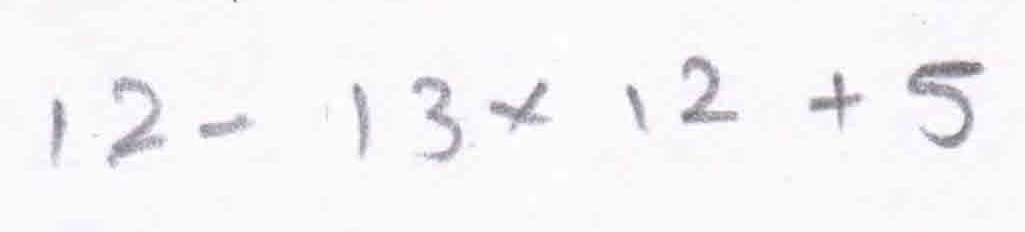
\includegraphics[width=3cm]{Q2_D117227_Math.png}}
    \end{minipage}
    \vspace{10pt}

    % Image: Q2_D117237_Math.png - Scaled height: 8.03mm
    \begin{minipage}{\linewidth}
    \RaggedRight\textbf{\tiny \highgreen{Cathrine Bertina F [C]}} \\ 
    \vspace{4.00pt}\fcolorbox{blue}{white}{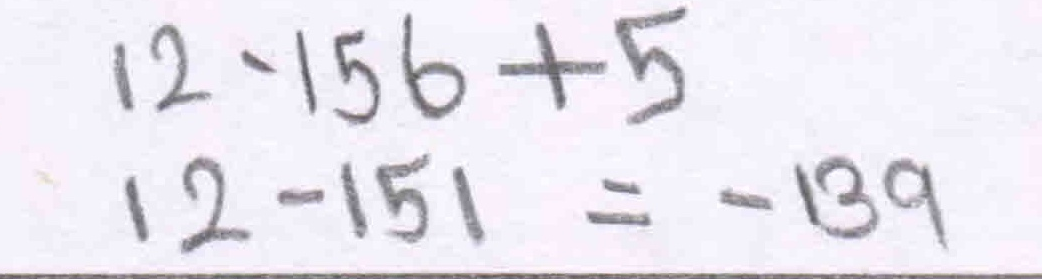
\includegraphics[width=3cm]{Q2_D117237_Math.png}}
    \end{minipage}
    \vspace{10pt}

    % Image: Q2_D117239_Math.png - Scaled height: 12.28mm
    \begin{minipage}{\linewidth}
    \RaggedRight\textbf{\tiny \highgreen{Inika N [C]}} \\ 
    \vspace{4.00pt}\fcolorbox{blue}{white}{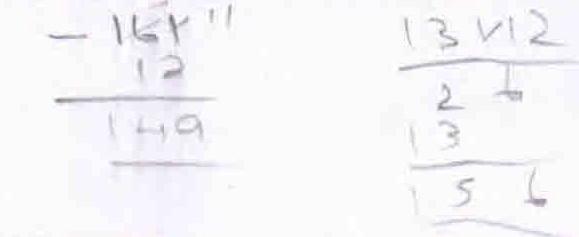
\includegraphics[width=3cm]{Q2_D117239_Math.png}}
    \end{minipage}
    \vspace{10pt}

    % Image: Q2_D117241_Math.png - Scaled height: 7.97mm
    \begin{minipage}{\linewidth}
    \RaggedRight\textbf{\tiny \highgreen{Nidharshana D [C]}} \\ 
    \vspace{4.00pt}\fcolorbox{blue}{white}{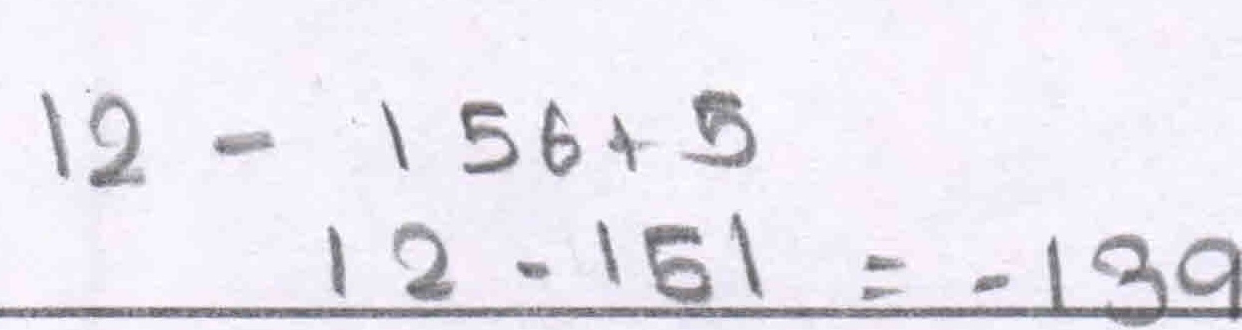
\includegraphics[width=3cm]{Q2_D117241_Math.png}}
    \end{minipage}
    \vspace{10pt}

    % Image: Q2_D117245_Math.png - Scaled height: 14.31mm
    \begin{minipage}{\linewidth}
    \RaggedRight\textbf{\tiny \highgreen{Sowbarnika S [C]}} \\ 
    \vspace{4.00pt}\fcolorbox{blue}{white}{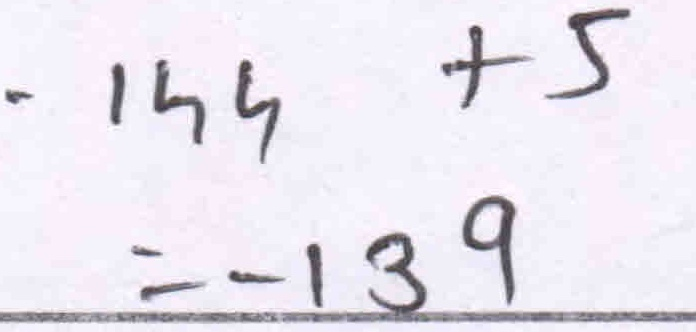
\includegraphics[width=3cm]{Q2_D117245_Math.png}}
    \end{minipage}
    \vspace{10pt}

    \end{multicols}
\end{frame}




\begin{frame}[shrink=0.1,label=QPC8QC6M01 - BM - Q4]{Q3 [Basic Math]}
\vspace{-0.2cm}
\mcqtextbottomOneFour{
questionnumber={3}, 
questionTag={C6M01 - BM - Q4}, 
questiontext={Express 15 cm in meters.},
optionA={15 m},
optionB={1500 m},
optionC={0.15 m},
optionD={100 m},
correctoption={C},}

\begin{minipage}{\linewidth}
\hspace{1cm}
\centering
\tiny
\renewcommand{\arraystretch}{1.25}
\begin{tabular}{|M{1.2cm}|M{0.8cm}|M{0.8cm}|M{0.8cm}|M{0.8cm}|M{0.8cm}|}
\hline
Option & A (\ding{55}) & B (\ding{55}) & \cellcolor{cellgreen} C (\ding{51}) & D (\ding{55}) & E \\ 
\hline
8 A & \highno{8\%} & \highno{69\%} & \highred{23\%} & \highno{0\%} & \highno{0\%} \\ 
 \hline 
8 B & \highno{0\%} & \highno{27\%} & \highno{73\%} & \highno{0\%} & \highno{0\%} \\ \hline
\end{tabular}
\end{minipage}

\end{frame}
% \input{4. PPT/6. My Answer/Math/C8/117_C8M - Q3}


\begin{frame}[shrink=0.1,label=QPC8QC7M07 - BM - Q1]{Q4 [Basic Math]}
\vspace{-0.2cm}
\mcqtextbottomOneFour{
questionnumber={4},
questionTag={C7M07 - BM - Q1},
questiontext={ Which equation is correct when $x$ = 5, $y$ = 10?    },
optionA={$2x=9y$},
optionB={$5x=y+5$},
optionC={$10x=5y$},
optionD={$5x+5 = 10y+10$},
correctoption={C},
}

\begin{minipage}{\linewidth}
\hspace{1cm}
\centering
\tiny
\renewcommand{\arraystretch}{1.25}
\begin{tabular}{|M{1.2cm}|M{0.8cm}|M{0.8cm}|M{0.8cm}|M{0.8cm}|M{0.8cm}|}
\hline
Option & A (\ding{55}) & B (\ding{55}) & \cellcolor{cellgreen} C (\ding{51}) & D (\ding{55}) & E \\ 
\hline
8 A & \highno{0\%} & \highno{23\%} & \highno{54\%} & \highno{8\%} & \highno{15\%} \\ 
 \hline 
8 B & \highno{0\%} & \highno{0\%} & \highgreen{100\%} & \highno{0\%} & \highno{0\%} \\ \hline
\end{tabular}
\end{minipage}

\end{frame}
% \input{4. PPT/6. My Answer/Math/C8/117_C8M - Q4}


\begin{frame}[shrink=0.1,label=QPC8QC6M04 - BM - Q3]{Q5 [Basic Math]}
\vspace{-0.2cm}
\mcqtextbottomOneFour{
questionnumber={5}, 
questionTag={C6M04 - BM - Q3}, 
questiontext={Find the LCM of 96, 64},
optionA={190},
optionB={192},
optionC={6144},
optionD={164},
correctoption={B},}

\begin{minipage}{\linewidth}
\hspace{1cm}
\centering
\tiny
\renewcommand{\arraystretch}{1.25}
\begin{tabular}{|M{1.2cm}|M{0.8cm}|M{0.8cm}|M{0.8cm}|M{0.8cm}|M{0.8cm}|}
\hline
Option & A (\ding{55}) & \cellcolor{cellgreen} B (\ding{51}) & C (\ding{55}) & D (\ding{55}) & E \\ 
\hline
8 A & \highno{0\%} & \highgreen{85\%} & \highno{15\%} & \highno{0\%} & \highno{0\%} \\ 
 \hline 
8 B & \highno{0\%} & \highgreen{87\%} & \highno{7\%} & \highno{7\%} & \highno{0\%} \\ \hline
\end{tabular}
\end{minipage}

\end{frame}
\begin{frame}{Q5 - My Answer Responses}
    \vspace{-0.6cm}
    \begin{multicols}{3}

    % Image: Q5_D117215_Math.png - Scaled height: 2.96mm
    \begin{minipage}{\linewidth}
    \RaggedRight\textbf{\tiny \highred{Dharun J [C]}} \\ 
    \vspace{4.00pt}\fcolorbox{blue}{white}{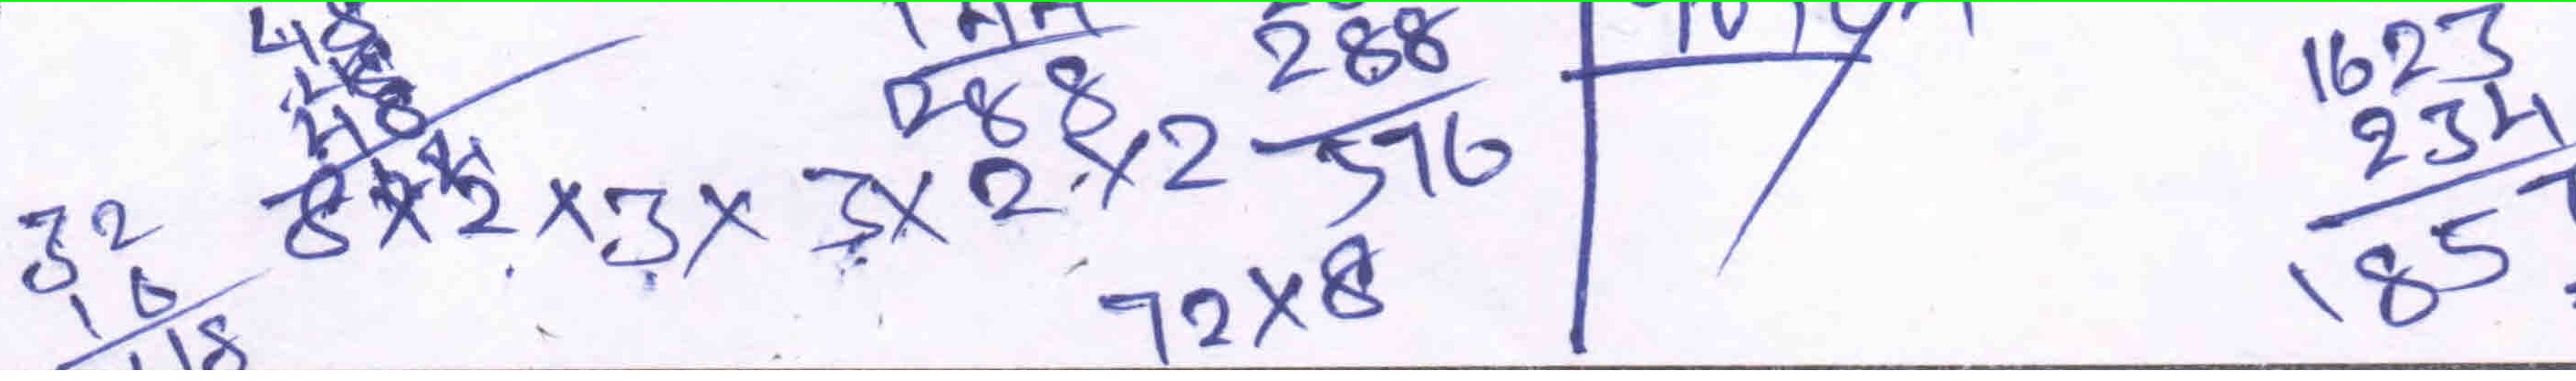
\includegraphics[width=4cm]{Q5_D117215_Math.png}}
    \end{minipage}
    \vspace{10pt}

    % Image: Q5_D117216_Math.png - Scaled height: 4.83mm
    \begin{minipage}{\linewidth}
    \RaggedRight\textbf{\tiny \highgreen{Dheavvarshan S S [B]}} \\ 
    \vspace{4.00pt}\fcolorbox{blue}{white}{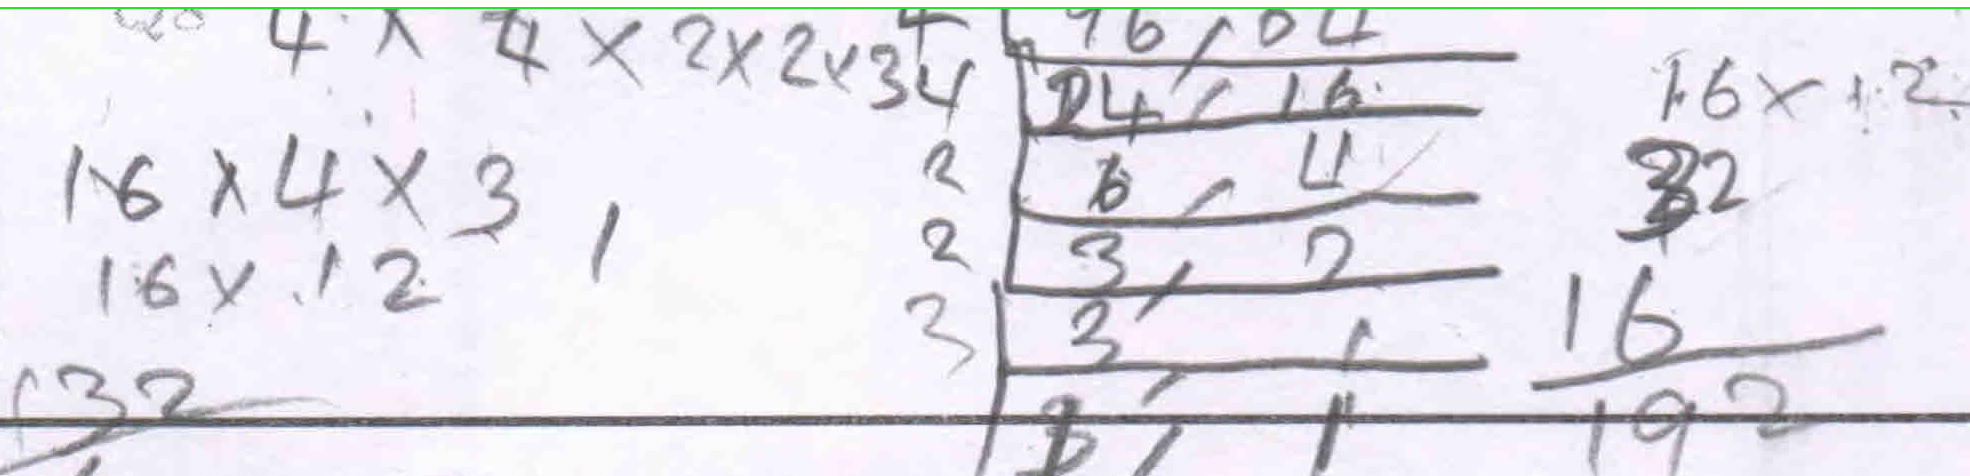
\includegraphics[width=4cm]{Q5_D117216_Math.png}}
    \end{minipage}
    \vspace{10pt}

    % Image: Q5_D117221_Math.png - Scaled height: 4.58mm
    \begin{minipage}{\linewidth}
    \RaggedRight\textbf{\tiny \highgreen{Dharani B [B]}} \\ 
    \vspace{4.00pt}\fcolorbox{blue}{white}{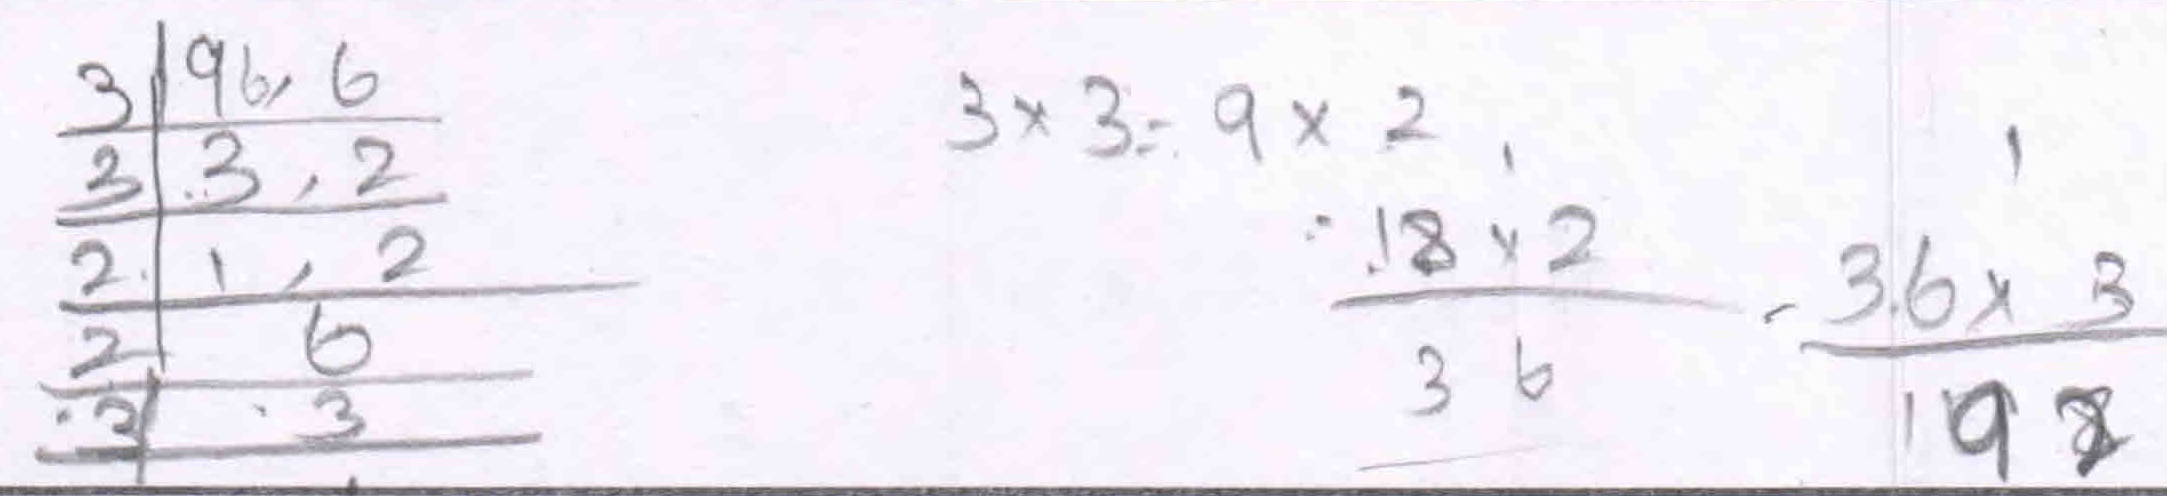
\includegraphics[width=4cm]{Q5_D117221_Math.png}}
    \end{minipage}
    \vspace{10pt}

    % Image: Q5_D117227_Math.png - Scaled height: 3.23mm
    \begin{minipage}{\linewidth}
    \RaggedRight\textbf{\tiny \highgreen{Subiksha P [B]}} \\ 
    \vspace{4.00pt}\fcolorbox{blue}{white}{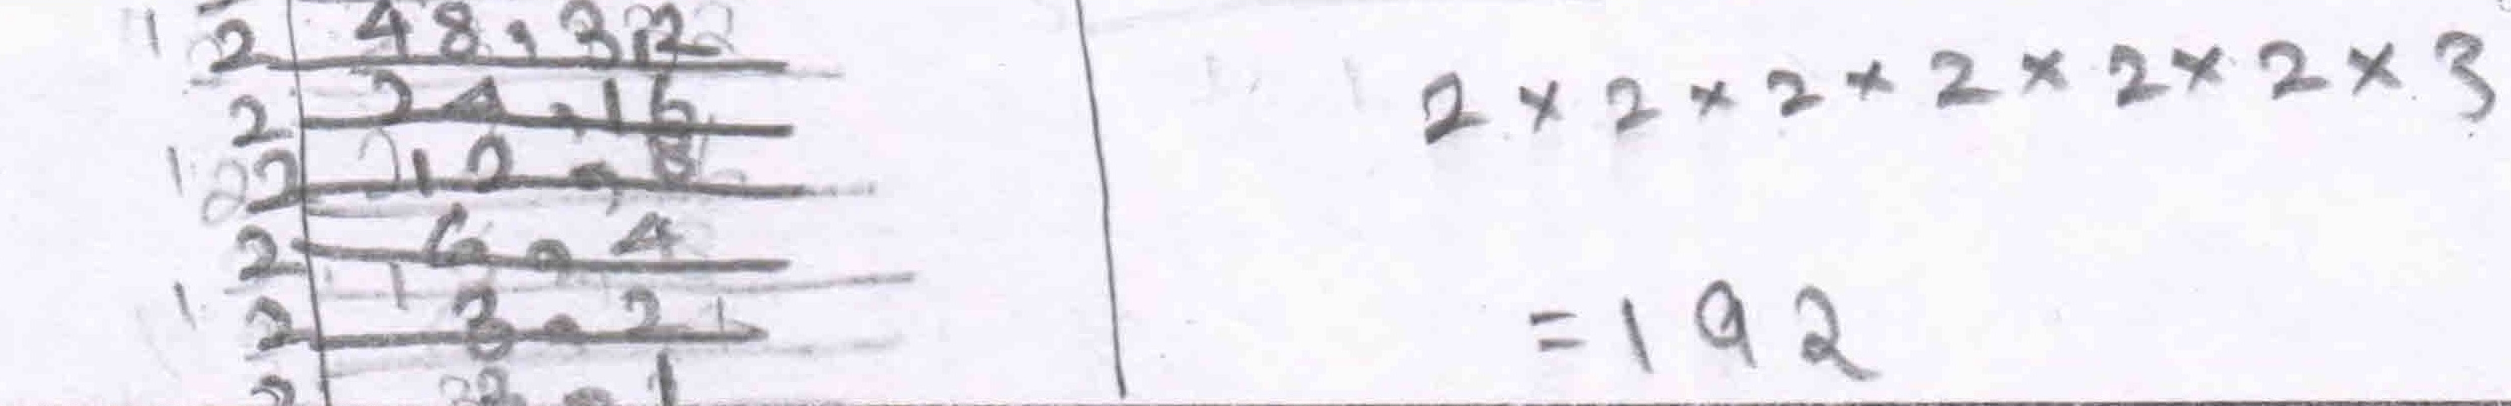
\includegraphics[width=4cm]{Q5_D117227_Math.png}}
    \end{minipage}
    \vspace{10pt}

    % Image: Q5_D117237_Math.png - Scaled height: 3.79mm
    \begin{minipage}{\linewidth}
    \RaggedRight\textbf{\tiny \highgreen{Cathrine Bertina F [B]}} \\ 
    \vspace{4.00pt}\fcolorbox{blue}{white}{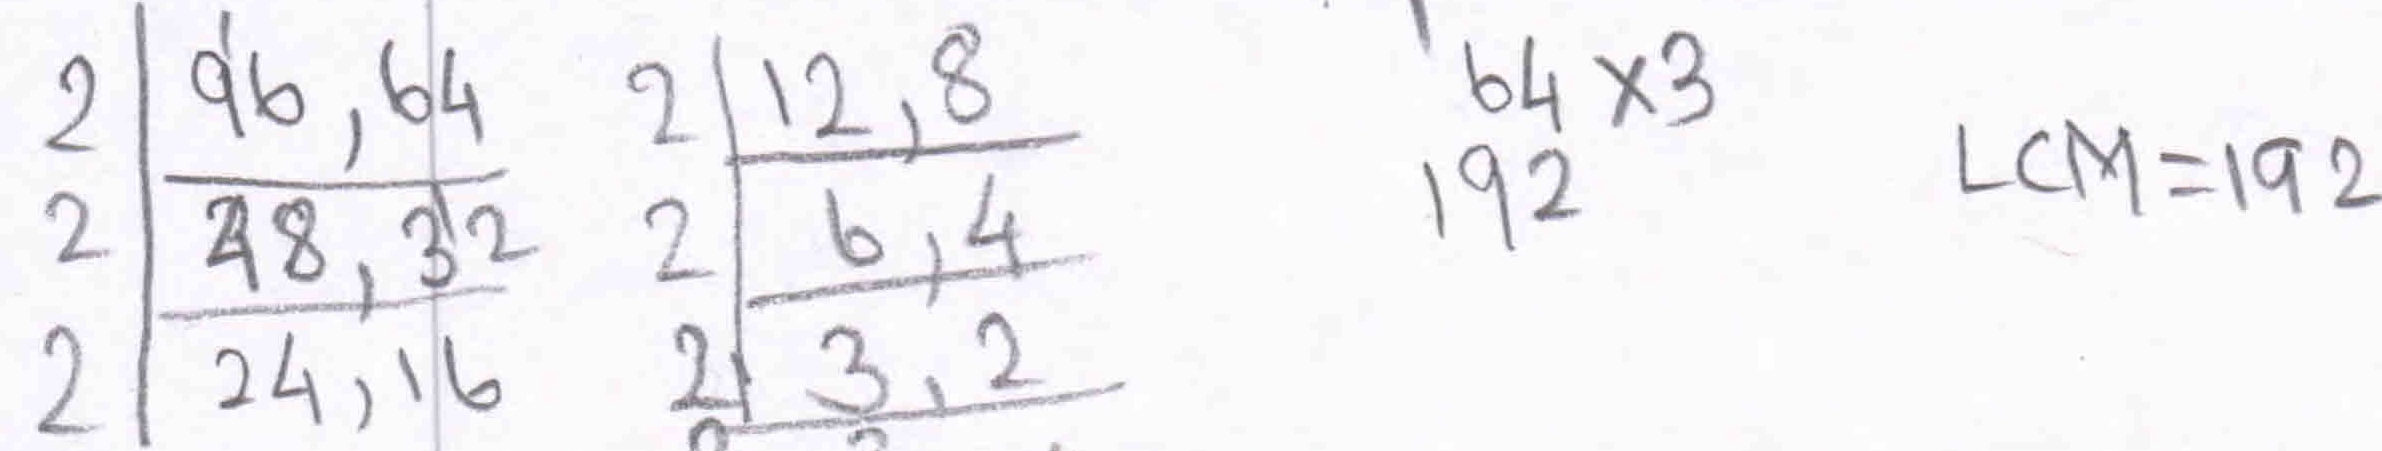
\includegraphics[width=4cm]{Q5_D117237_Math.png}}
    \end{minipage}
    \vspace{10pt}

    % Image: Q5_D117239_Math.png - Scaled height: 5.30mm
    \begin{minipage}{\linewidth}
    \RaggedRight\textbf{\tiny \highgreen{Inika N [B]}} \\ 
    \vspace{4.00pt}\fcolorbox{blue}{white}{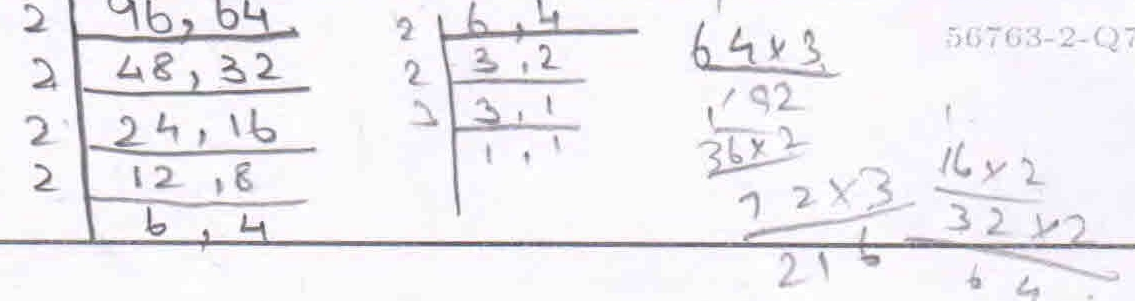
\includegraphics[width=4cm]{Q5_D117239_Math.png}}
    \end{minipage}
    \vspace{10pt}

    % Image: Q5_D117241_Math.png - Scaled height: 5.84mm
    \begin{minipage}{\linewidth}
    \RaggedRight\textbf{\tiny \highgreen{Nidharshana D [B]}} \\ 
    \vspace{4.00pt}\fcolorbox{blue}{white}{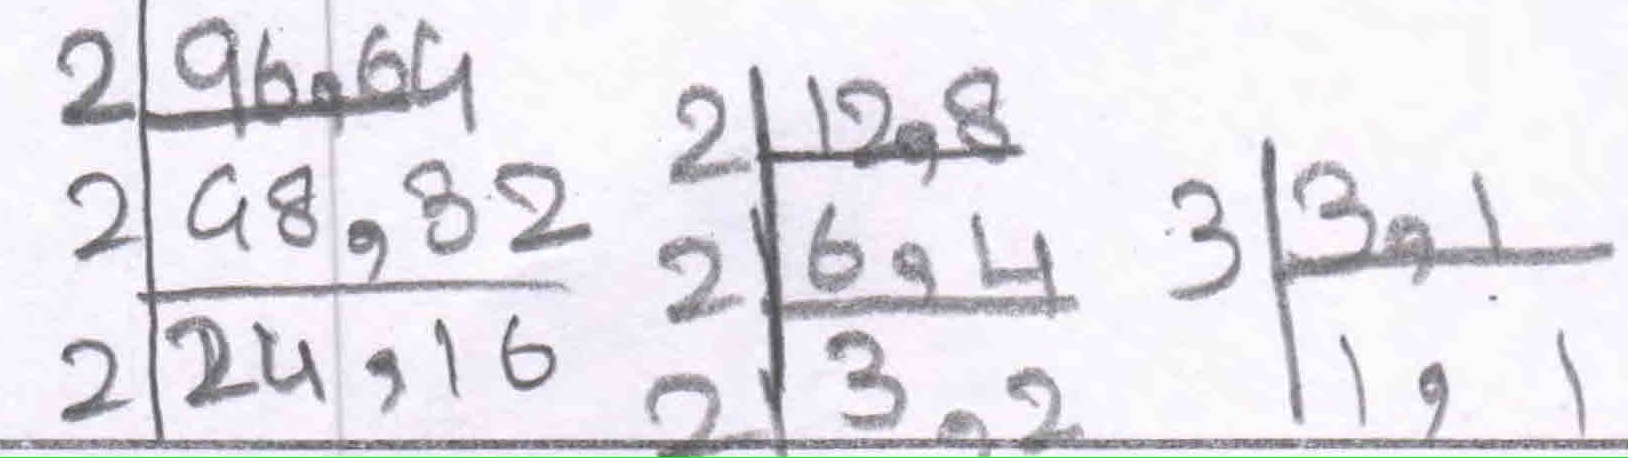
\includegraphics[width=4cm]{Q5_D117241_Math.png}}
    \end{minipage}
    \vspace{10pt}

    % Image: Q5_D117244_Math.png - Scaled height: 3.82mm
    \begin{minipage}{\linewidth}
    \RaggedRight\textbf{\tiny \highgreen{Shamyuktha Y [B]}} \\ 
    \vspace{4.00pt}\fcolorbox{blue}{white}{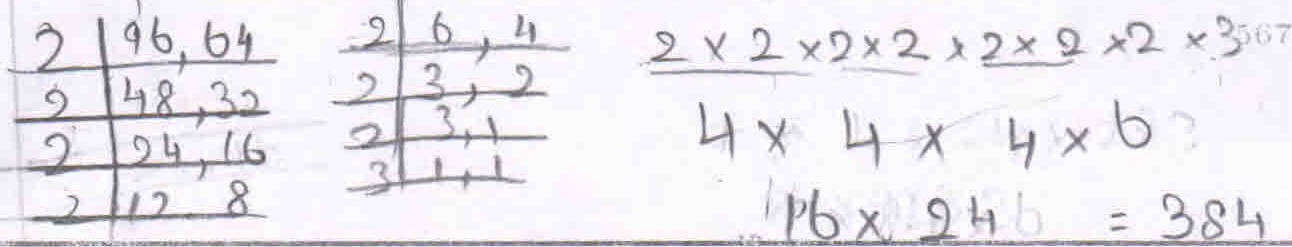
\includegraphics[width=4cm]{Q5_D117244_Math.png}}
    \end{minipage}
    \vspace{10pt}

    % Image: Q5_D117245_Math.png - Scaled height: 4.47mm
    \begin{minipage}{\linewidth}
    \RaggedRight\textbf{\tiny \highgreen{Sowbarnika S [B]}} \\ 
    \vspace{4.00pt}\fcolorbox{blue}{white}{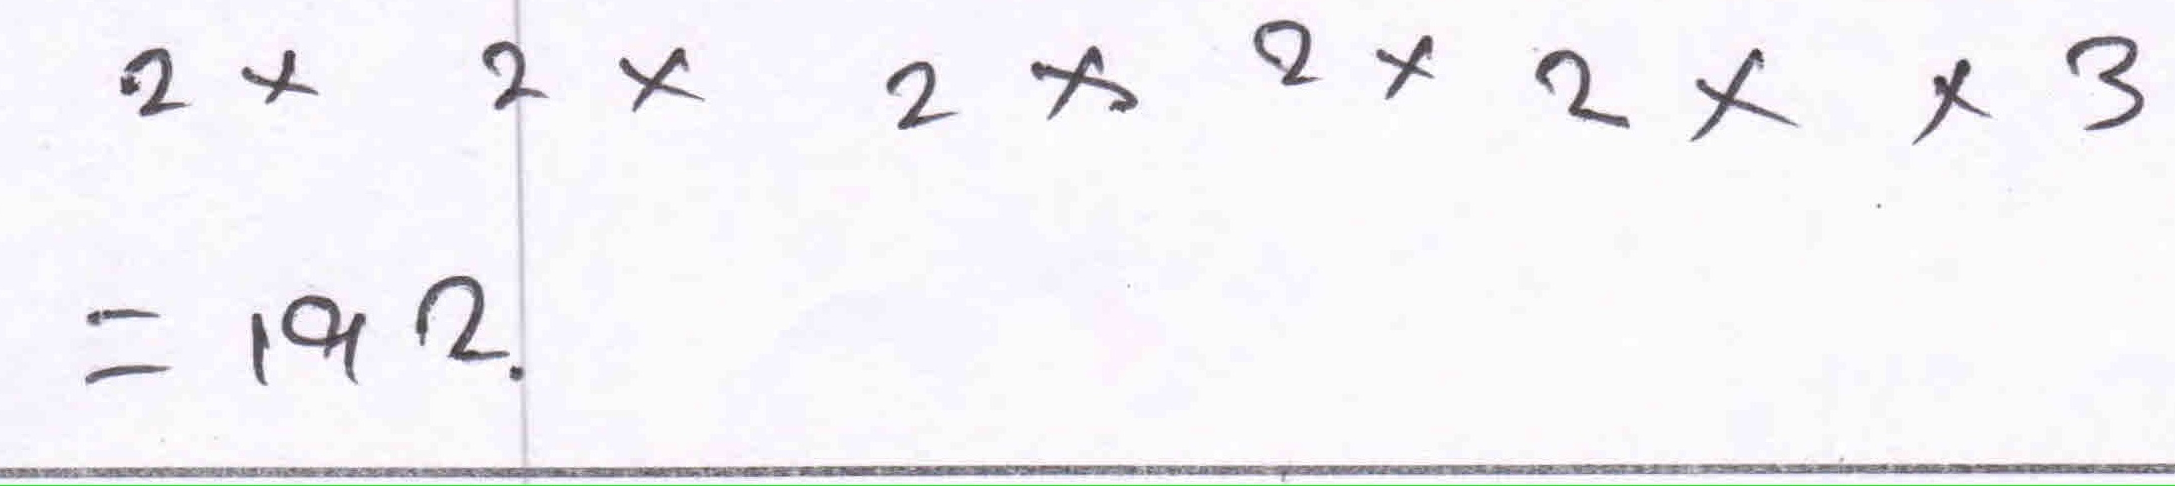
\includegraphics[width=4cm]{Q5_D117245_Math.png}}
    \end{minipage}
    \vspace{10pt}

    \end{multicols}
\end{frame}




\begin{frame}[shrink=0.1,label=QPC8QC6M01 - BM - Q2]{Q6 [Basic Math]}
\vspace{-0.2cm}
\mcqtextbottomOneFour{
questionnumber={6}, 
questionTag={C6M01 - BM - Q2}, 
questiontext={Add the following.\\
\qquad  i. Ninety-nine lakhs seventy thousand seven hundred and eighty-one.\\
\qquad  ii. Nine lakh five hundred and one.},
optionA={1,49,97,831},
optionB={99,80,281},
optionC={1,08,71,282},
optionD={1,89,71,282},
correctoption={C},
}

\begin{minipage}{\linewidth}
\hspace{1cm}
\centering
\tiny
\renewcommand{\arraystretch}{1.25}
\begin{tabular}{|M{1.2cm}|M{0.8cm}|M{0.8cm}|M{0.8cm}|M{0.8cm}|M{0.8cm}|}
\hline
Option & A (\ding{55}) & B (\ding{55}) & \cellcolor{cellgreen} C (\ding{51}) & D (\ding{55}) & E \\ 
\hline
8 A & \highno{15\%} & \highno{8\%} & \highgreen{77\%} & \highno{0\%} & \highno{0\%} \\ 
 \hline 
8 B & \highno{0\%} & \highno{7\%} & \highgreen{93\%} & \highno{0\%} & \highno{0\%} \\ \hline
\end{tabular}
\end{minipage}

\end{frame}
% \input{4. PPT/6. My Answer/Math/C8/117_C8M - Q6}


\begin{frame}[shrink=0.1,label=QPC8QC6M01 - BM - Q3]{Q7 [Basic Math]}
\vspace{-0.2cm}
\mcqimgleftFourOne{
questionnumber={7}, 
questionTag={C6M01 - BM - Q3},
questiontext={Subtract the following.},
imgtabletikz = {
\begin{table}[H]
\centering
\renewcommand{\arraystretch}{1.3}
\begin{tabular}{ccccccc}
&2 &4 &6 &4 &6 &7  \\
($-$) &1&2&4&7&5&7 \\
\hline
&&&&&&\\
\hline
\end{tabular}
\end{table}
},
optionA={371224},
optionB={121710},
optionC={100111},
optionD={122293},
correctoption={B},
leftmini={0.5},
rightmini={0.4},
}

\begin{minipage}{\linewidth}
\hspace{1cm}
\centering
\tiny
\renewcommand{\arraystretch}{1.25}
\begin{tabular}{|M{1.2cm}|M{0.8cm}|M{0.8cm}|M{0.8cm}|M{0.8cm}|M{0.8cm}|}
\hline
Option & A (\ding{55}) & \cellcolor{cellgreen} B (\ding{51}) & C (\ding{55}) & D (\ding{55}) & E \\ 
\hline
8 A & \highno{0\%} & \highgreen{92\%} & \highno{0\%} & \highno{0\%} & \highno{8\%} \\ 
 \hline 
8 B & \highno{7\%} & \highgreen{93\%} & \highno{0\%} & \highno{0\%} & \highno{0\%} \\ \hline
\end{tabular}
\end{minipage}

\end{frame}
% \input{4. PPT/6. My Answer/Math/C8/117_C8M - Q7}


\begin{frame}[shrink=0.1,label=QPC8QC7M16 - BM - Q1]{Q8 [Basic Math]}
\vspace{-0.2cm}
\mcqtextbottomOneFour{
questionnumber={8}, 
questionTag={C7M16 - BM - Q1}, 
questiontext={Find the area of the parallelogram if the base and height are 14 cm and 7.4 cm respectively.},
optionA={21.4 sq. cm},
optionB={ 51.8 sq. cm},
optionC={103.6 sq. cm},
optionD={147.4  sq. units},
correctoption={C},
}

\begin{minipage}{\linewidth}
\hspace{1cm}
\centering
\tiny
\renewcommand{\arraystretch}{1.25}
\begin{tabular}{|M{1.2cm}|M{0.8cm}|M{0.8cm}|M{0.8cm}|M{0.8cm}|M{0.8cm}|}
\hline
Option & A (\ding{55}) & B (\ding{55}) & \cellcolor{cellgreen} C (\ding{51}) & D (\ding{55}) & E \\ 
\hline
8 A & \highno{23\%} & \highno{15\%} & \highred{38\%} & \highno{23\%} & \highno{0\%} \\ 
 \hline 
8 B & \highno{7\%} & \highno{40\%} & \highno{47\%} & \highno{0\%} & \highno{7\%} \\ \hline
\end{tabular}
\end{minipage}

\end{frame}
% \input{4. PPT/6. My Answer/Math/C8/117_C8M - Q8}


\begin{frame}[shrink=0.1,label=QPC8QC6M07 - BM - Q3]{Q9 [Basic Math]}
\vspace{-0.2cm}
\mcqtextbottomOneFour{
questionnumber={9},
questionTag={C6M07 - BM - Q3},
questiontext={Add: 234.55 + 1623.4},
optionA={396.89},
optionB={3968.9},
optionC={1857.59},
optionD={1857.95},
correctoption={D},
}

\begin{minipage}{\linewidth}
\hspace{1cm}
\centering
\tiny
\renewcommand{\arraystretch}{1.25}
\begin{tabular}{|M{1.2cm}|M{0.8cm}|M{0.8cm}|M{0.8cm}|M{0.8cm}|M{0.8cm}|}
\hline
Option & A (\ding{55}) & B (\ding{55}) & C (\ding{55}) & \cellcolor{cellgreen} D (\ding{51}) & E \\ 
\hline
8 A & \highno{8\%} & \highno{31\%} & \highno{23\%} & \highred{31\%} & \highno{8\%} \\ 
 \hline 
8 B & \highno{7\%} & \highno{7\%} & \highno{33\%} & \highno{53\%} & \highno{0\%} \\ \hline
\end{tabular}
\end{minipage}

\end{frame}
\begin{frame}{Q9 - My Answer Responses}
    \vspace{-0.6cm}
    \begin{multicols}{4}

    

    % Image: Q9_D117215_Math.png - Scaled height: 9.95mm
    \begin{minipage}{\linewidth}
    \RaggedRight\textbf{\tiny \highred{Dharun J [C]}} \\ 
    \vspace{4.00pt}\fcolorbox{blue}{white}{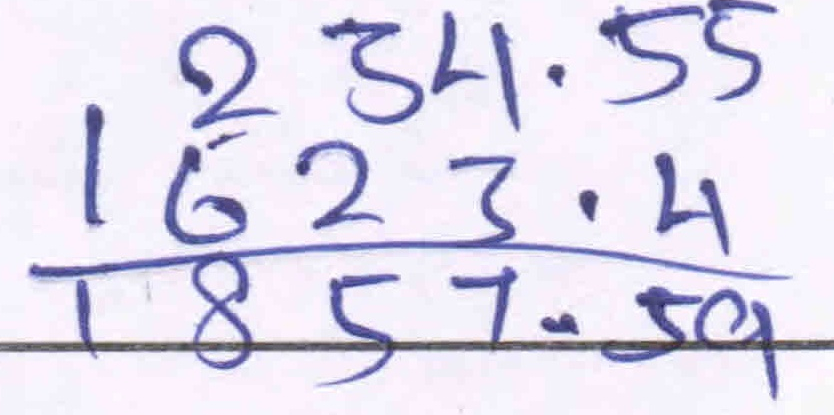
\includegraphics[width=2cm]{Q9_D117215_Math.png}}
    \end{minipage}
    \vspace{10pt}

    % Image: Q9_D117216_Math.png - Scaled height: 8.41mm
    \begin{minipage}{\linewidth}
    \RaggedRight\textbf{\tiny \highred{Dheavvarshan S S [B]}} \\ 
    \vspace{4.00pt}\fcolorbox{blue}{white}{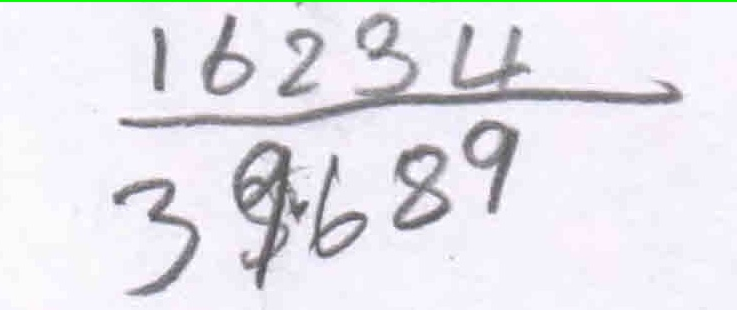
\includegraphics[width=2cm]{Q9_D117216_Math.png}}
    \end{minipage}
    \vspace{10pt}

    % Image: Q9_D117220_Math.png - Scaled height: 10.82mm
    \begin{minipage}{\linewidth}
    \RaggedRight\textbf{\tiny \highgreen{Vipulan J R [D]}} \\ 
    \vspace{4.00pt}\fcolorbox{blue}{white}{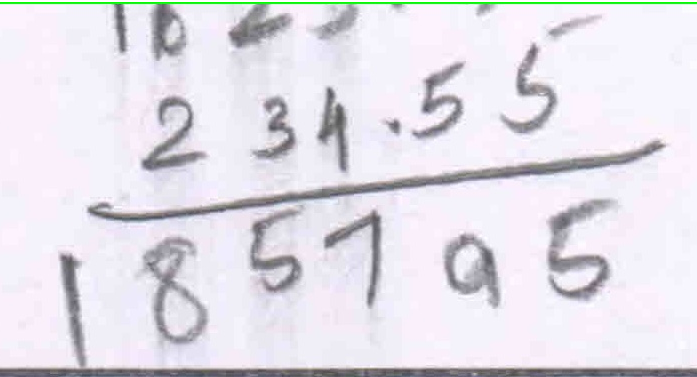
\includegraphics[width=2cm]{Q9_D117220_Math.png}}
    \end{minipage}
    \vspace{10pt}

    % Image: Q9_D117222_Math.png - Scaled height: 7.56mm
    \begin{minipage}{\linewidth}
    \RaggedRight\textbf{\tiny \highred{Ilakiya R S []}} \\ 
    \vspace{4.00pt}\fcolorbox{blue}{white}{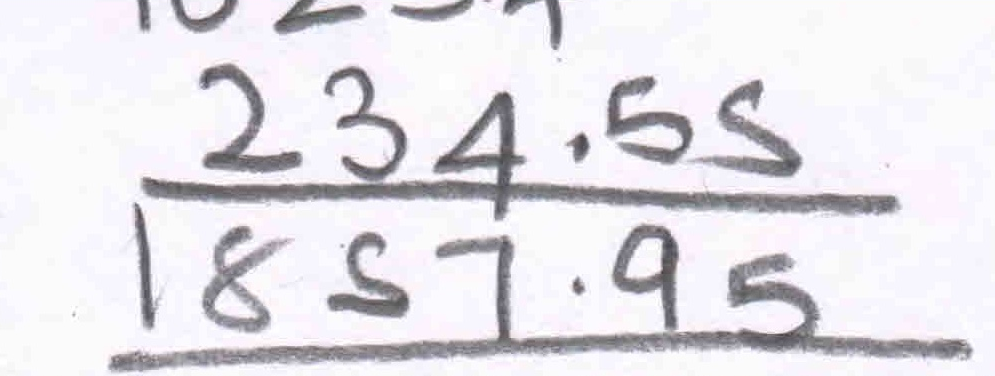
\includegraphics[width=2cm]{Q9_D117222_Math.png}}
    \end{minipage}
    \vspace{10pt}

    % Image: Q9_D117226_Math.png - Scaled height: 4.12mm
    \begin{minipage}{\linewidth}
    \RaggedRight\textbf{\tiny \highgreen{Oviya M S [D]}} \\ 
    \vspace{4.00pt}\fcolorbox{blue}{white}{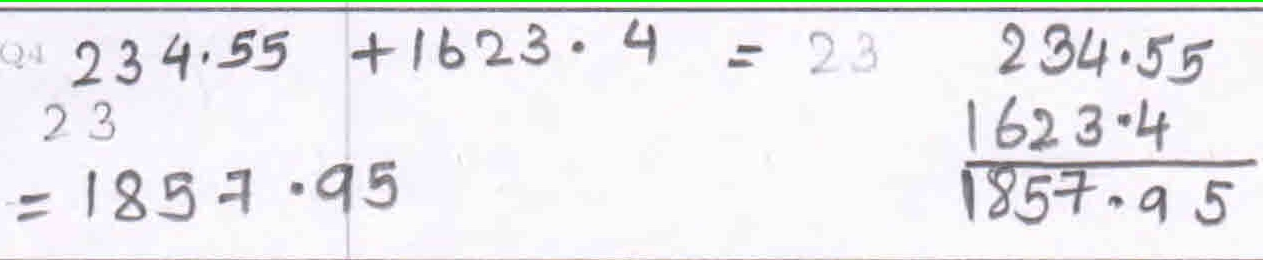
\includegraphics[width=2cm]{Q9_D117226_Math.png}}
    \end{minipage}
    \vspace{10pt}

    % Image: Q9_D117227_Math.png - Scaled height: 6.91mm
    \begin{minipage}{\linewidth}
    \RaggedRight\textbf{\tiny \highgreen{Subiksha P [D]}} \\ 
    \vspace{4.00pt}\fcolorbox{blue}{white}{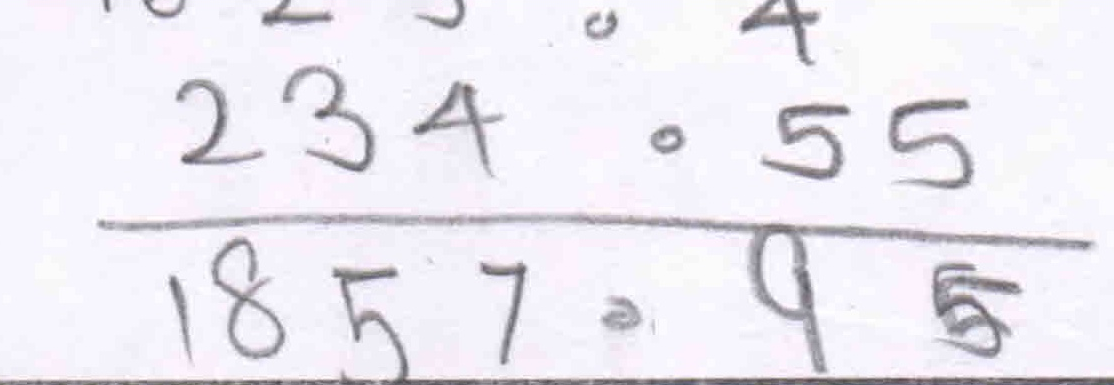
\includegraphics[width=2cm]{Q9_D117227_Math.png}}
    \end{minipage}
    \vspace{10pt}

    % Image: Q9_D117232_Math.png - Scaled height: 11.61mm
    \begin{minipage}{\linewidth}
    \RaggedRight\textbf{\tiny \highred{Logabalaji S [B]}} \\ 
    \vspace{4.00pt}\fcolorbox{blue}{white}{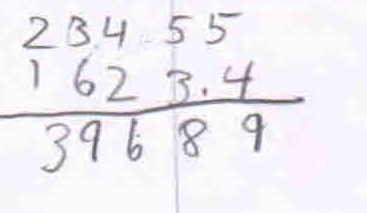
\includegraphics[width=2cm]{Q9_D117232_Math.png}}
    \end{minipage}
    \vspace{10pt}

    % Image: Q9_D117236_Math.png - Scaled height: 6.95mm
    \begin{minipage}{\linewidth}
    \RaggedRight\textbf{\tiny \highgreen{Anushka M [D]}} \\ 
    \vspace{4.00pt}\fcolorbox{blue}{white}{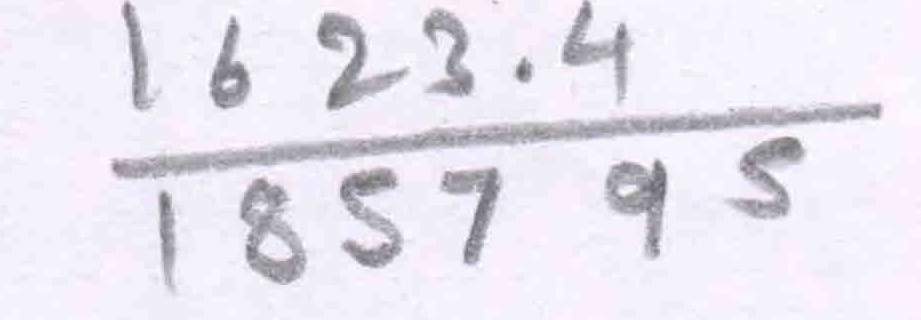
\includegraphics[width=2cm]{Q9_D117236_Math.png}}
    \end{minipage}
    \vspace{10pt}

    % Image: Q9_D117237_Math.png - Scaled height: 7.13mm
    \begin{minipage}{\linewidth}
    \RaggedRight\textbf{\tiny \highgreen{Cathrine Bertina F [D]}} \\ 
    \vspace{4.00pt}\fcolorbox{blue}{white}{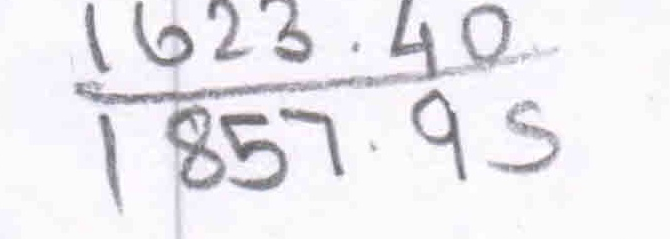
\includegraphics[width=2cm]{Q9_D117237_Math.png}}
    \end{minipage}
    \vspace{10pt}

    % Image: Q9_D117239_Math.png - Scaled height: 6.08mm
    \begin{minipage}{\linewidth}
    \RaggedRight\textbf{\tiny \highgreen{Inika N [D]}} \\ 
    \vspace{4.00pt}\fcolorbox{blue}{white}{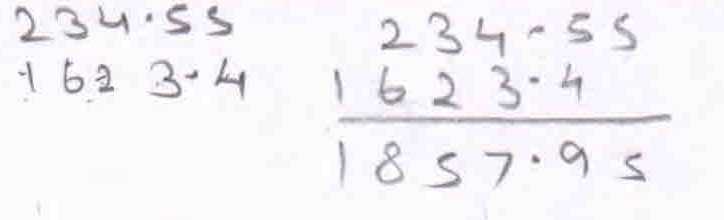
\includegraphics[width=2cm]{Q9_D117239_Math.png}}
    \end{minipage}
    \vspace{10pt}

    % Image: Q9_D117244_Math.png - Scaled height: 10.36mm
    \begin{minipage}{\linewidth}
    \RaggedRight\textbf{\tiny \highgreen{Shamyuktha Y [D]}} \\ 
    \vspace{4.00pt}\fcolorbox{blue}{white}{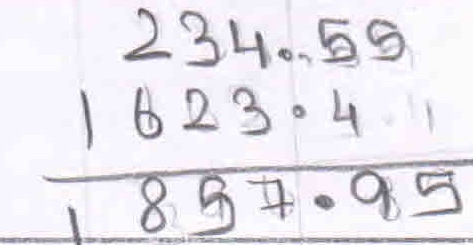
\includegraphics[width=2cm]{Q9_D117244_Math.png}}
    \end{minipage}
    \vspace{10pt}

    % Image: Q9_D117250_Math.png - Scaled height: 7.81mm
    \begin{minipage}{\linewidth}
    \RaggedRight\textbf{\tiny \highred{Tharshan K [B]}} \\ 
    \vspace{4.00pt}\fcolorbox{blue}{white}{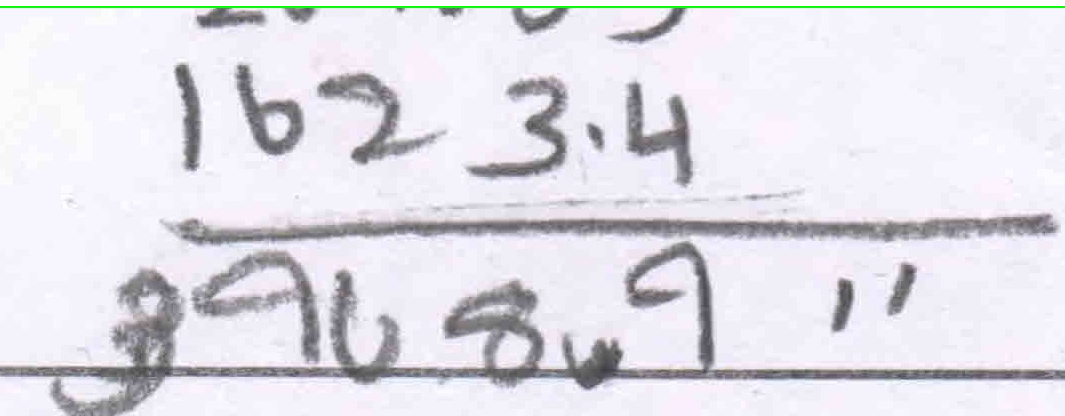
\includegraphics[width=2cm]{Q9_D117250_Math.png}}
    \end{minipage}
    \vspace{10pt}

    \end{multicols}
\end{frame}




\begin{frame}[shrink=0.1,label=QPC8QC6M11 - BM - Q1]{Q10 [Basic Math]}
\vspace{-0.2cm}
\mcqimgleftFourOne{
questionnumber={10}, 
questionTag={C6M11 - BM - Q1}, 
questiontext={The number of angles formed inside the given figure is \rule{80pt}{0.5pt}.},
imgtabletikz ={
\tikzset{every picture/.style={line width=0.75pt,scale=\scalefactor}} 
\begin{tikzpicture}[x=0.75pt,y=0.75pt,yscale=-1,xscale=1]
\draw   (100,126) -- (259,126) -- (259,216.86) -- (100,216.86) -- cycle ;
\end{tikzpicture}
},
optionA={2},
optionB={3},
optionC={4},
optionD={8},
correctoption={C},
leftmini={0.5},
rightmini={0.4},}

\begin{minipage}{\linewidth}
\hspace{1cm}
\centering
\tiny
\renewcommand{\arraystretch}{1.25}
\begin{tabular}{|M{1.2cm}|M{0.8cm}|M{0.8cm}|M{0.8cm}|M{0.8cm}|M{0.8cm}|}
\hline
Option & A (\ding{55}) & B (\ding{55}) & \cellcolor{cellgreen} C (\ding{51}) & D (\ding{55}) & E \\ 
\hline
8 A & \highno{0\%} & \highno{0\%} & \highgreen{85\%} & \highno{8\%} & \highno{8\%} \\ 
 \hline 
8 B & \highno{0\%} & \highno{0\%} & \highgreen{93\%} & \highno{7\%} & \highno{0\%} \\ \hline
\end{tabular}
\end{minipage}

\end{frame}
% \input{4. PPT/6. My Answer/Math/C8/117_C8M - Q10}


\begin{frame}[shrink=0.1,label=QPC8QC5BM - BM - Q11]{Q11 [Basic Math]}
\vspace{-0.2cm}
\mcqtextbottomOneFour{
questionnumber={11}, 
questionTag={C5BM - BM - Q11}, 
questiontext={A movie theater screens 195 shows in 65 days. Identify the number of shows to be screened in a day by dividing the total number of shows by the total number of days.},
optionA={64},
optionB={2},
optionC={3},
optionD={130},
correctoption={C},}

\begin{minipage}{\linewidth}
\hspace{1cm}
\centering
\tiny
\renewcommand{\arraystretch}{1.25}
\begin{tabular}{|M{1.2cm}|M{0.8cm}|M{0.8cm}|M{0.8cm}|M{0.8cm}|M{0.8cm}|}
\hline
Option & A (\ding{55}) & B (\ding{55}) & \cellcolor{cellgreen} C (\ding{51}) & D (\ding{55}) & E \\ 
\hline
8 A & \highno{0\%} & \highno{23\%} & \highno{69\%} & \highno{0\%} & \highno{8\%} \\ 
 \hline 
8 B & \highno{7\%} & \highno{7\%} & \highgreen{87\%} & \highno{0\%} & \highno{0\%} \\ \hline
\end{tabular}
\end{minipage}

\end{frame}
% \input{4. PPT/6. My Answer/Math/C8/117_C8M - Q11}


\begin{frame}[shrink=0.1,label=QPC8QC8M01 - DT - Q4]{Q13 [1. Rational Numbers]}
\vspace{-0.2cm}
\mcqtextbottomOneFour{
questionnumber={13}, 
questionTag={C8M01 - DT - Q4}, 
questiontext={Which of the following is not a rational number?},
optionA={-2},
optionB={{{$\dfrac{0}{2}$}}},
optionC={0},
optionD={{{$\dfrac{2}{0}$}}},
correctoption={D},
}

\begin{minipage}{\linewidth}
\hspace{1cm}
\centering
\tiny
\renewcommand{\arraystretch}{1.25}
\begin{tabular}{|M{1.2cm}|M{0.8cm}|M{0.8cm}|M{0.8cm}|M{0.8cm}|M{0.8cm}|}
\hline
Option & A (\ding{55}) & B (\ding{55}) & C (\ding{55}) & \cellcolor{cellgreen} D (\ding{51}) & E \\ 
\hline
8 A & \highno{23\%} & \highno{8\%} & \highno{15\%} & \highno{46\%} & \highno{8\%} \\ 
 \hline 
8 B & \highno{7\%} & \highno{0\%} & \highno{7\%} & \highgreen{80\%} & \highno{7\%} \\ \hline
\end{tabular}
\end{minipage}

\end{frame}
% \input{4. PPT/6. My Answer/Math/C8/117_C8M - Q13}


\begin{frame}[shrink=0.1,label=QPC8QC8M01 - DT - Q5]{Q46 [1. Rational Numbers]}
\vspace{-0.2cm}
\mcqimgleftFourOne{
questionnumber={46}, 
questionTag={C8M01 - DT - Q5},
questiontext={Separate positive and negative rational numbers. Which type of number is more frequent?},
imgtabletikz = {
\tikzset{every picture/.style={line width=0.75pt,scale=\scalefactor}} 
\begin{tikzpicture}[x=0.75pt,y=0.75pt,yscale=-1,xscale=1] 
\draw   (104,53) -- (434,53) -- (434,169) -- (104,169) -- cycle ;
\draw (126,70) node [anchor=north west][inner sep=0.75pt]   [align=left] {$\dfrac{4}{5}$};
\draw (189,70) node [anchor=north west][inner sep=0.75pt]   [align=left] {$\dfrac{3}{7}$};
\draw (248,70) node [anchor=north west][inner sep=0.75pt]   [align=left] {$\dfrac{-1}{1}$};
\draw (305,70) node [anchor=north west][inner sep=0.75pt]   [align=left] {$\dfrac{1}{0}$};
\draw (362,70) node [anchor=north west][inner sep=0.75pt]   [align=left] {$\dfrac{1}{7}$};
\draw (148,120) node [anchor=north west][inner sep=0.75pt]   [align=left] {$-\dfrac{9}{7}$};
\draw (226,120) node [anchor=north west][inner sep=0.75pt]   [align=left] {$-\dfrac{2}{3}$};
\draw (300,120) node [anchor=north west][inner sep=0.75pt]   [align=left] {$-\dfrac{3}{7}$};
\draw (375,120) node [anchor=north west][inner sep=0.75pt]   [align=left] {$\dfrac{9}{5}$};
\end{tikzpicture}},
optionA={ Positive rational numbers},
optionB={Negative rational numbers},
optionC={ Both are equal},
optionD={Cannot be determined},
correctoption={C},
leftmini={0.5},
rightmini={0.4},
}

\begin{minipage}{\linewidth}
\hspace{1cm}
\centering
\tiny
\renewcommand{\arraystretch}{1.25}
\begin{tabular}{|M{1.2cm}|M{0.8cm}|M{0.8cm}|M{0.8cm}|M{0.8cm}|M{0.8cm}|}
\hline
Option & A (\ding{55}) & B (\ding{55}) & \cellcolor{cellgreen} C (\ding{51}) & D (\ding{55}) & E \\ 
\hline
8 A & \highno{62\%} & \highno{8\%} & \highred{23\%} & \highno{0\%} & \highno{8\%} \\ 
 \hline 
8 B & \highno{47\%} & \highno{7\%} & \highno{47\%} & \highno{0\%} & \highno{0\%} \\ \hline
\end{tabular}
\end{minipage}

\end{frame}
% \input{4. PPT/6. My Answer/Math/C8/117_C8M - Q46}


\begin{frame}[shrink=0.1,label=QPC8QC8M01 - DT - Q9]{Q55 [1. Rational Numbers]}
\vspace{-0.2cm}
\mcqtextbottomTwoTwo{
questionnumber={55}, 
questionTag={C8M01 - DT - Q9}, 
questiontext={Match the following.\\ \smallskip
\renewcommand{\arraystretch}{1.75}
\begin{tabular}{|p{0.25cm}|p{5cm}|p{0.25cm}|p{0.25cm}|p{5cm}|}
\hline
\multicolumn{2}{|c|}{Column A} & & \multicolumn{2}{|c|}{Column B} \\
\cline{1-2}\cline{4-5}
i & Associative property  & & a& {{$\dfrac{1}{2}$}} $\times$ {{$\dfrac{1}{3}$}} = {{$\dfrac{1}{3}$}} $\times$ {{$\dfrac{1}{2}$}}\\
\cline{1-2}\cline{4-5}
ii & Closure property   & & b & {{$\dfrac{1}{2}$}} - {{$\dfrac{1}{3}$}} $\longrightarrow$ Rational number \\
\cline{1-2}\cline{4-5}
iii & Commutative property & & c& {{$\dfrac{1}{2}$}} $\times$ ({{$\dfrac{1}{3}$}} $\times$ {{$\dfrac{1}{4}$}}) = ({{$\dfrac{1}{2}$}} $\times$ {{$\dfrac{1}{3}$}}) $\times$ {{$\dfrac{1}{4}$}} \\
\cline{1-2}\cline{4-5}
iv & Distributive property  & & d & {{$\dfrac{1}{2}$}} $\times$ ({{$\dfrac{1}{3}$}} + {{$\dfrac{1}{4}$}}) = ({{$\dfrac{1}{2}$}} $\times$ {{$\dfrac{1}{3}$}}) + ({{$\dfrac{1}{2}$}} $\times$ {{$\dfrac{1}{4}$}}) \\
\hline
\end{tabular}
},
optionA={ i - a, ii - b, iii - c, iv - d},
optionB={ i - c, ii - b, iii - a, iv - d},
optionC={ i - b, ii - a, iii - c, iv - d},
optionD={ i - b, ii - c, iii - d, iv - a},
correctoption={B},
}

\begin{minipage}{\linewidth}
\hspace{1cm}
\centering
\tiny
\renewcommand{\arraystretch}{1.25}
\begin{tabular}{|M{1.2cm}|M{0.8cm}|M{0.8cm}|M{0.8cm}|M{0.8cm}|M{0.8cm}|}
\hline
Option & A (\ding{55}) & \cellcolor{cellgreen} B (\ding{51}) & C (\ding{55}) & D (\ding{55}) & E \\ 
\hline
8 A & \highno{23\%} & \highno{46\%} & \highno{0\%} & \highno{31\%} & \highno{0\%} \\ 
 \hline 
8 B & \highno{13\%} & \highgreen{80\%} & \highno{7\%} & \highno{0\%} & \highno{0\%} \\ \hline
\end{tabular}
\end{minipage}

\end{frame}
\begin{frame}{Q55 - My Answer Responses}
    \vspace{-0.6cm}
    \begin{multicols}{2}

    % Image: Q55_D117215_Math.png - Scaled height: 3.47mm
    \begin{minipage}{\linewidth}
    \RaggedRight\textbf{\tiny \highred{Dharun J [D]}} \\ 
    \vspace{4.00pt}\fcolorbox{blue}{white}{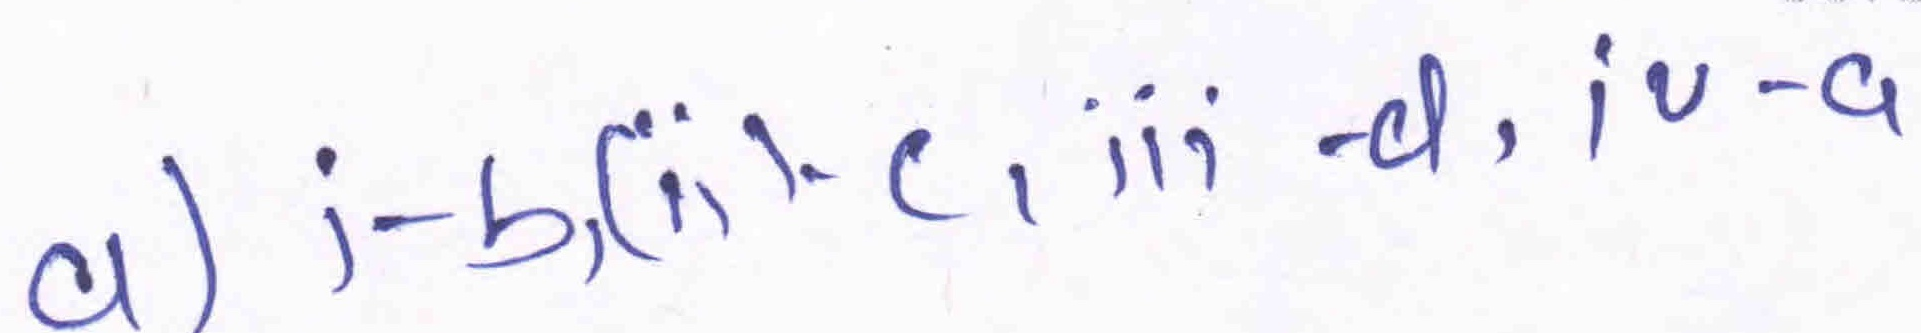
\includegraphics[width=4cm]{Q55_D117215_Math.png}}
    \end{minipage}
    \vspace{10pt}

    % Image: Q55_D117222_Math.png - Scaled height: 3.71mm
    \begin{minipage}{\linewidth}
    \RaggedRight\textbf{\tiny \highred{Ilakiya R S [A]}} \\ 
    \vspace{4.00pt}\fcolorbox{blue}{white}{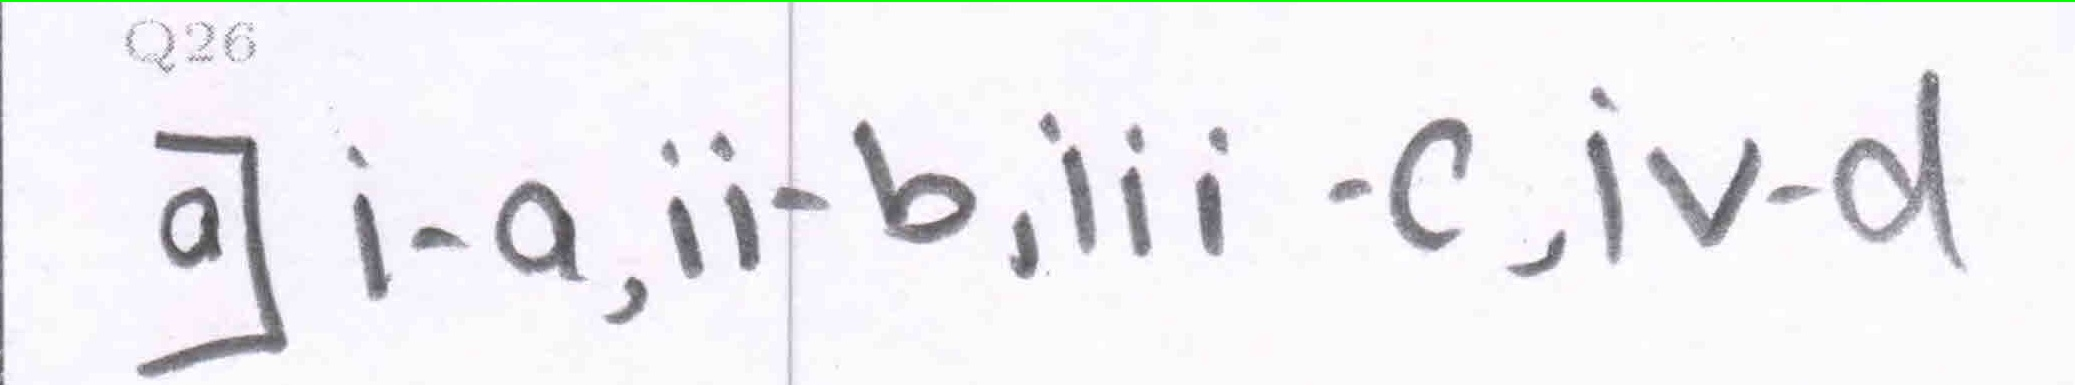
\includegraphics[width=4cm]{Q55_D117222_Math.png}}
    \end{minipage}
    \vspace{10pt}

    % Image: Q55_D117226_Math.png - Scaled height: 2.62mm
    \begin{minipage}{\linewidth}
    \RaggedRight\textbf{\tiny \highgreen{Oviya M S [B]}} \\ 
    \vspace{4.00pt}\fcolorbox{blue}{white}{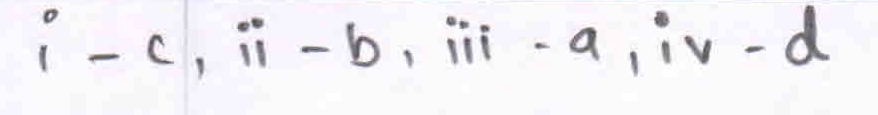
\includegraphics[width=4cm]{Q55_D117226_Math.png}}
    \end{minipage}
    \vspace{10pt}

    % Image: Q55_D117239_Math.png - Scaled height: 3.56mm
    \begin{minipage}{\linewidth}
    \RaggedRight\textbf{\tiny \highgreen{Inika N [B]}} \\ 
    \vspace{4.00pt}\fcolorbox{blue}{white}{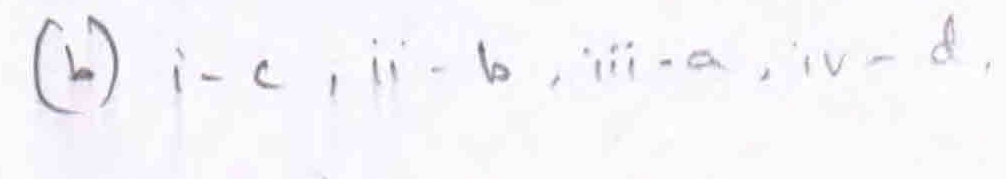
\includegraphics[width=4cm]{Q55_D117239_Math.png}}
    \end{minipage}
    \vspace{10pt}

    % Image: Q55_D117242_Math.png - Scaled height: 2.13mm
    \begin{minipage}{\linewidth}
    \RaggedRight\textbf{\tiny \highgreen{Pranavi T [B]}} \\ 
    \vspace{4.00pt}\fcolorbox{blue}{white}{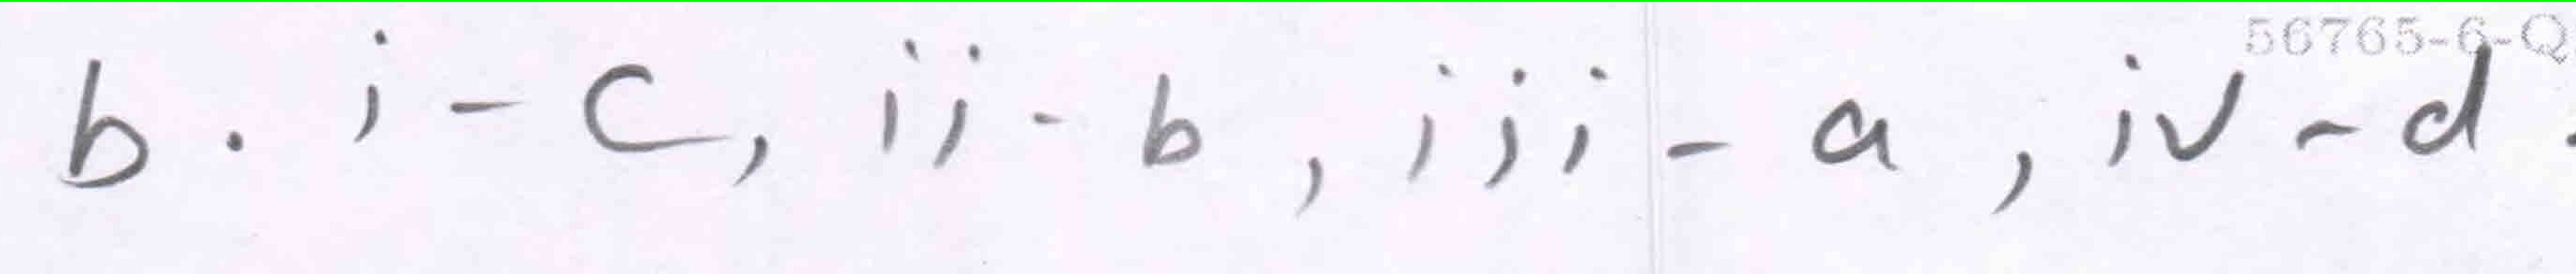
\includegraphics[width=4cm]{Q55_D117242_Math.png}}
    \end{minipage}
    \vspace{10pt}

    \end{multicols}
\end{frame}




\begin{frame}[shrink=0.1,label=QPC8QC8M01 - CT - Q1]{Q60 [1. Rational Numbers]}
\vspace{-0.2cm}
\mcqtextbottomOneFour{
questionnumber={60 - Critical Thinking},
questionTag={C8M01 - CT - Q1},
questiontext={Find the value of  B - A from the following.\\ (Hint: The given square is a magical square, where the sum of each row, column and diagonal are the same.) 
\begin{table}[H]
\centering
\renewcommand{\arraystretch}{2}
\begin{tabular}{|p{1cm}|p{1cm}|p{1cm}|}
\hline
\Centering {{$\dfrac{4}{5}$}} & \Centering {{$\dfrac{9}{5}$}} & \Centering  {{$\dfrac{2}{5}$}}  \\
\hline
\Centering {{$\dfrac{A}{5}$}} & \Centering 1 &  \Centering {{$\dfrac{B}{5}$}}  \\
\hline
\Centering {{$\dfrac{8}{5}$}} & \Centering {{$\dfrac{1}{5}$}} & \Centering  {{$\dfrac{6}{5}$}}  \\
\hline
\end{tabular}
\end{table} 
},
optionA={3},
optionB={4},
optionC={7},
optionD={0},
correctoption={B},
}

\begin{minipage}{\linewidth}
\hspace{1cm}
\centering
\tiny
\renewcommand{\arraystretch}{1.25}
\begin{tabular}{|M{1.2cm}|M{0.8cm}|M{0.8cm}|M{0.8cm}|M{0.8cm}|M{0.8cm}|}
\hline
Option & A (\ding{55}) & \cellcolor{cellgreen} B (\ding{51}) & C (\ding{55}) & D (\ding{55}) & E \\ 
\hline
8 A & \highno{0\%} & \highred{38\%} & \highno{46\%} & \highno{0\%} & \highno{15\%} \\ 
 \hline 
8 B & \highno{7\%} & \highno{60\%} & \highno{27\%} & \highno{0\%} & \highno{7\%} \\ \hline
\end{tabular}
\end{minipage}

\end{frame}
% \input{4. PPT/6. My Answer/Math/C8/117_C8M - Q60 - Critical Thinking}


\begin{frame}[shrink=0.1,label=QPC8QC8M07 - DT - Q2]{Q20 [2. Linear Equations in One Variable]}
\vspace{-0.2cm}
\mcqtextbottomOneFour{
questionnumber={20}, 
questionTag={C8M07 - DT - Q2}, 
questiontext={Which of the following equation is correct when $x$ = 4?},
optionA={7 - 2$x$ = 1},
optionB={13$x$ = 52},
optionC={44$x$},
optionD={ {{$\dfrac{x}{4}$}} + 20 = 22},
correctoption={B},
}

\begin{minipage}{\linewidth}
\hspace{1cm}
\centering
\tiny
\renewcommand{\arraystretch}{1.25}
\begin{tabular}{|M{1.2cm}|M{0.8cm}|M{0.8cm}|M{0.8cm}|M{0.8cm}|M{0.8cm}|}
\hline
Option & A (\ding{55}) & \cellcolor{cellgreen} B (\ding{51}) & C (\ding{55}) & D (\ding{55}) & E \\ 
\hline
8 A & \highno{38\%} & \highred{31\%} & \highno{31\%} & \highno{0\%} & \highno{0\%} \\ 
 \hline 
8 B & \highno{7\%} & \highgreen{93\%} & \highno{0\%} & \highno{0\%} & \highno{0\%} \\ \hline
\end{tabular}
\end{minipage}

\end{frame}
% \input{4. PPT/6. My Answer/Math/C8/117_C8M - Q20}


\begin{frame}[shrink=0.1,label=QPC8QC8M07 - DT - Q3]{Q22 [2. Linear Equations in One Variable]}
\vspace{-0.2cm}
\mcqtextbottomOneFour{
questionnumber={22}, 
questionTag={C8M07 - DT - Q3}, 
questiontext={Identify the linear equation in one variable.\\ \smallskip
\hspace{1cm} i. $x^2 + x =12$ \hspace{1cm} ii. $5z+3=130$ \hspace{1cm} iii. $v^2+h^3=12$ },
optionA={i, ii},
optionB={ii},
optionC={ii, iii},
optionD={All the above},
correctoption={B},
}

\begin{minipage}{\linewidth}
\hspace{1cm}
\centering
\tiny
\renewcommand{\arraystretch}{1.25}
\begin{tabular}{|M{1.2cm}|M{0.8cm}|M{0.8cm}|M{0.8cm}|M{0.8cm}|M{0.8cm}|}
\hline
Option & A (\ding{55}) & \cellcolor{cellgreen} B (\ding{51}) & C (\ding{55}) & D (\ding{55}) & E \\ 
\hline
8 A & \highno{31\%} & \highno{46\%} & \highno{0\%} & \highno{23\%} & \highno{0\%} \\ 
 \hline 
8 B & \highno{0\%} & \highgreen{87\%} & \highno{0\%} & \highno{7\%} & \highno{7\%} \\ \hline
\end{tabular}
\end{minipage}

\end{frame}
% \input{4. PPT/6. My Answer/Math/C8/117_C8M - Q22}


\begin{frame}[shrink=0.1,label=QPC8QC8M07 - DT - Q6]{Q35 [2. Linear Equations in One Variable]}
\vspace{-0.2cm}
\mcqtextbottomOneFour{
questionnumber={35}, 
questionTag={C8M07 - DT - Q6}, 
questiontext={Solve the given equation. {{$\dfrac{x}{4}$}} $ - 5 = $ {{$\dfrac{x}{2}$}}    },
optionA={$-$20},
optionB={{{$\dfrac{4}{5}$}}},
optionC={$-$ {{$\dfrac{9}{2}$}} },
optionD={$-$10},
correctoption={A},
}

\begin{minipage}{\linewidth}
\hspace{1cm}
\centering
\tiny
\renewcommand{\arraystretch}{1.25}
\begin{tabular}{|M{1.2cm}|M{0.8cm}|M{0.8cm}|M{0.8cm}|M{0.8cm}|M{0.8cm}|}
\hline
Option & \cellcolor{cellgreen} A (\ding{51}) & B (\ding{55}) & C (\ding{55}) & D (\ding{55}) & E \\ 
\hline
8 A & \highred{38\%} & \highno{15\%} & \highno{8\%} & \highno{31\%} & \highno{8\%} \\ 
 \hline 
8 B & \highno{67\%} & \highno{0\%} & \highno{7\%} & \highno{27\%} & \highno{0\%} \\ \hline
\end{tabular}
\end{minipage}

\end{frame}
% \input{4. PPT/6. My Answer/Math/C8/117_C8M - Q35}


\begin{frame}[shrink=0.1,label=QPC8QC8M07 - DT - Q1]{Q53 [2. Linear Equations in One Variable]}
\vspace{-0.2cm}
\mcqtextbottomOneFour{
questionnumber={53}, 
questionTag={C8M07 - DT - Q1}, 
questiontext={Which of the following cannot be a part of the expression?},
optionA={Variables},
optionB={  Constants},
optionC={Equal to sign},
optionD={Both a and b},
correctoption={C},
}

\begin{minipage}{\linewidth}
\hspace{1cm}
\centering
\tiny
\renewcommand{\arraystretch}{1.25}
\begin{tabular}{|M{1.2cm}|M{0.8cm}|M{0.8cm}|M{0.8cm}|M{0.8cm}|M{0.8cm}|}
\hline
Option & A (\ding{55}) & B (\ding{55}) & \cellcolor{cellgreen} C (\ding{51}) & D (\ding{55}) & E \\ 
\hline
8 A & \highno{15\%} & \highno{0\%} & \highno{54\%} & \highno{8\%} & \highno{23\%} \\ 
 \hline 
8 B & \highno{13\%} & \highno{0\%} & \highgreen{80\%} & \highno{0\%} & \highno{7\%} \\ \hline
\end{tabular}
\end{minipage}

\end{frame}
% \input{4. PPT/6. My Answer/Math/C8/117_C8M - Q53}


\begin{frame}[shrink=0.1,label=QPC8QC8M12 - DT - Q7]{Q28 [3. Understanding Quadrilaterals]}
\vspace{-0.2cm}
\mcqtextbottomOneFour{
questionnumber={28}, 
questionTag={C8M12 - DT - Q7}, 
questiontext={Find the quadrilateral with all the interior angles as 90$^\circ$.},
optionA={Rectangle},
optionB={Rhombus},
optionC={Parallelogram},
optionD={Triangle},
correctoption={A},
}

\begin{minipage}{\linewidth}
\hspace{1cm}
\centering
\tiny
\renewcommand{\arraystretch}{1.25}
\begin{tabular}{|M{1.2cm}|M{0.8cm}|M{0.8cm}|M{0.8cm}|M{0.8cm}|M{0.8cm}|}
\hline
Option & \cellcolor{cellgreen} A (\ding{51}) & B (\ding{55}) & C (\ding{55}) & D (\ding{55}) & E \\ 
\hline
8 A & \highred{38\%} & \highno{8\%} & \highno{23\%} & \highno{23\%} & \highno{8\%} \\ 
 \hline 
8 B & \highno{73\%} & \highno{13\%} & \highno{0\%} & \highno{13\%} & \highno{0\%} \\ \hline
\end{tabular}
\end{minipage}

\end{frame}
% \input{4. PPT/6. My Answer/Math/C8/117_C8M - Q28}


\begin{frame}[shrink=0.1,label=QPC8QC8M12 - DT - Q6]{Q36 [3. Understanding Quadrilaterals]}
\vspace{-0.2cm}
\mcqtextbottomTwoTwo{
questionnumber={36}, 
questionTag={C8M12 - DT - Q6}, 
questiontext={Match the following.\\
\begin{minipage}{0.4\textwidth}
\tikzset{every picture/.style={line width=0.75pt,scale=\scalefactor}}
\begin{tikzpicture}[x=0.75pt,y=0.75pt,yscale=-1,xscale=1]
\draw  [color={rgb, 255:red, 0; green, 0; blue, 0 }  ,draw opacity=1 ] (284.1,100) -- (408,100) -- (354.9,189) -- (231,189) -- cycle ;
\draw (271,85) node [anchor=north west][inner sep=0.75pt]   [align=left] {P};
\draw (406,85) node [anchor=north west][inner sep=0.75pt]   [align=left] {Q};
\draw (356.9,192) node [anchor=north west][inner sep=0.75pt]   [align=left] {R};
\draw (211.9,185) node [anchor=north west][inner sep=0.75pt]   [align=left] {S};
\end{tikzpicture}
\end{minipage}
\begin{minipage}{0.4\textwidth}
\renewcommand{\arraystretch}{1.25}
\begin{tabular}{|p{0.25cm}|p{3cm}|p{0.25cm}|p{0.25cm}|p{3cm}|}
\hline
\multicolumn{2}{|c|}{Column A} & & \multicolumn{2}{|c|}{Column B
} \\
\cline{1-2}\cline{4-5}
i & Opposite sides & & a & $\angle$R and $\angle$Q\\
\cline{1-2}\cline{4-5}
ii & Opposite angles  & & b & RS and QR \\
\cline{1-2}\cline{4-5}
iii & Adjacent sides   & & c & $\angle$S and $\angle$Q\\
\cline{1-2}\cline{4-5}
iv & Adjacent angles   & & d & PS and QR\\
\hline
\end{tabular} 
\end{minipage}},
optionA={i - c, ii - d, iii - a, iv - b},
optionB={i - d, ii - c, iii - b, iv - a},
optionC={i - d, ii - b, iii - a, iv - c},
optionD={i - b, ii - a, iii - d, iv - c},
correctoption={B},
}

\begin{minipage}{\linewidth}
\hspace{1cm}
\centering
\tiny
\renewcommand{\arraystretch}{1.25}
\begin{tabular}{|M{1.2cm}|M{0.8cm}|M{0.8cm}|M{0.8cm}|M{0.8cm}|M{0.8cm}|}
\hline
Option & A (\ding{55}) & \cellcolor{cellgreen} B (\ding{51}) & C (\ding{55}) & D (\ding{55}) & E \\ 
\hline
8 A & \highno{23\%} & \highno{54\%} & \highno{15\%} & \highno{8\%} & \highno{0\%} \\ 
 \hline 
8 B & \highno{7\%} & \highgreen{80\%} & \highno{7\%} & \highno{7\%} & \highno{0\%} \\ \hline
\end{tabular}
\end{minipage}

\end{frame}
% \input{4. PPT/6. My Answer/Math/C8/117_C8M - Q36}


\begin{frame}[shrink=0.1,label=QPC8QC8M12 - DT - Q1]{Q38 [3. Understanding Quadrilaterals]}
\vspace{-0.2cm}
\mcqimgleftFourOne{
questionnumber={38}, 
questionTag={C8M12 - DT - Q1},
questiontext={Match the following.},
imgtabletikz = {\renewcommand{\arraystretch}{1.25}
\begin{tabular}{|p{0.25cm}|p{3cm}|p{0.25cm}|p{0.25cm}|p{2cm}|}
\hline
\multicolumn{2}{|c|}{Shapes} & & \multicolumn{2}{|c|}{Number of sides} \\
\cline{1-2}\cline{4-5}
i & Heptagon & & a & 8\\
\cline{1-2}\cline{4-5}
ii & Octagon  & & b & 5 \\
\cline{1-2}\cline{4-5}
iii & Nonagon  & & c & 7\\
\cline{1-2}\cline{4-5}
iv & Pentagon  & & d & 9\\
\hline
\end{tabular}},
optionA={i - c, ii - a, iii - d, iv - b},
optionB={i - d, ii - b, iii - a, iv - c},
optionC={i - c, ii - d , iii - b, iv - a},
optionD={i - b, ii - a, iii - c, iv - d},
correctoption={A},
leftmini={0.5},
rightmini={0.4},
}

\begin{minipage}{\linewidth}
\hspace{1cm}
\centering
\tiny
\renewcommand{\arraystretch}{1.25}
\begin{tabular}{|M{1.2cm}|M{0.8cm}|M{0.8cm}|M{0.8cm}|M{0.8cm}|M{0.8cm}|}
\hline
Option & \cellcolor{cellgreen} A (\ding{51}) & B (\ding{55}) & C (\ding{55}) & D (\ding{55}) & E \\ 
\hline
8 A & \highgreen{85\%} & \highno{8\%} & \highno{0\%} & \highno{8\%} & \highno{0\%} \\ 
 \hline 
8 B & \highgreen{80\%} & \highno{7\%} & \highno{7\%} & \highno{7\%} & \highno{0\%} \\ \hline
\end{tabular}
\end{minipage}

\end{frame}
% \input{4. PPT/6. My Answer/Math/C8/117_C8M - Q38}


\begin{frame}[shrink=0.1,label=QPC8QC8M12 - CT - Q1]{Q59 [3. Understanding Quadrilaterals]}
\vspace{-0.2cm}
\mcqtextbottomOneFour{
questionnumber={59 - Critical Thinking},
questionTag = {C8M12 - CT - Q1},
questiontext = {Draw the rectangle and connect the parallel points based on the given conditions.\\
\qquad 1. ABCD is a rectangle.\\
\qquad 2. K, L, M and N are the midpoints of the sides AB, BC, CD and AD respectively.\\
\qquad 3. U is the midpoint of AK, and V is the midpoint of KB.\\
\qquad 4. X is the midpoint of MD, and W is the midpoint of CM.\\
\qquad 5. AU = AN \\
How many squares are formed in the rectangle AVWD?},
optionA={4},
optionB={1},
optionC={8},
optionD={12},
correctoption = {C},
}

\begin{minipage}{\linewidth}
\hspace{1cm}
\centering
\tiny
\renewcommand{\arraystretch}{1.25}
\begin{tabular}{|M{1.2cm}|M{0.8cm}|M{0.8cm}|M{0.8cm}|M{0.8cm}|M{0.8cm}|}
\hline
Option & A (\ding{55}) & B (\ding{55}) & \cellcolor{cellgreen} C (\ding{51}) & D (\ding{55}) & E \\ 
\hline
8 A & \highno{15\%} & \highno{31\%} & \highred{15\%} & \highno{31\%} & \highno{8\%} \\ 
 \hline 
8 B & \highno{20\%} & \highno{20\%} & \highred{33\%} & \highno{13\%} & \highno{13\%} \\ \hline
\end{tabular}
\end{minipage}

\end{frame}
% \input{4. PPT/6. My Answer/Math/C8/117_C8M - Q59 - Critical Thinking}


\begin{frame}[shrink=0.1,label=QPC8QC8M18 - DT - Q9]{Q37 [4. Data Handling]}
\vspace{-0.2cm}
\mcqtextbottomOneFour{
questionnumber={37}, 
questionTag={C8M18 - DT - Q9},
questiontext={What is the probability of getting an apple?\\ \hspace{3cm}
\adjustbox{scale=\scalefactor}{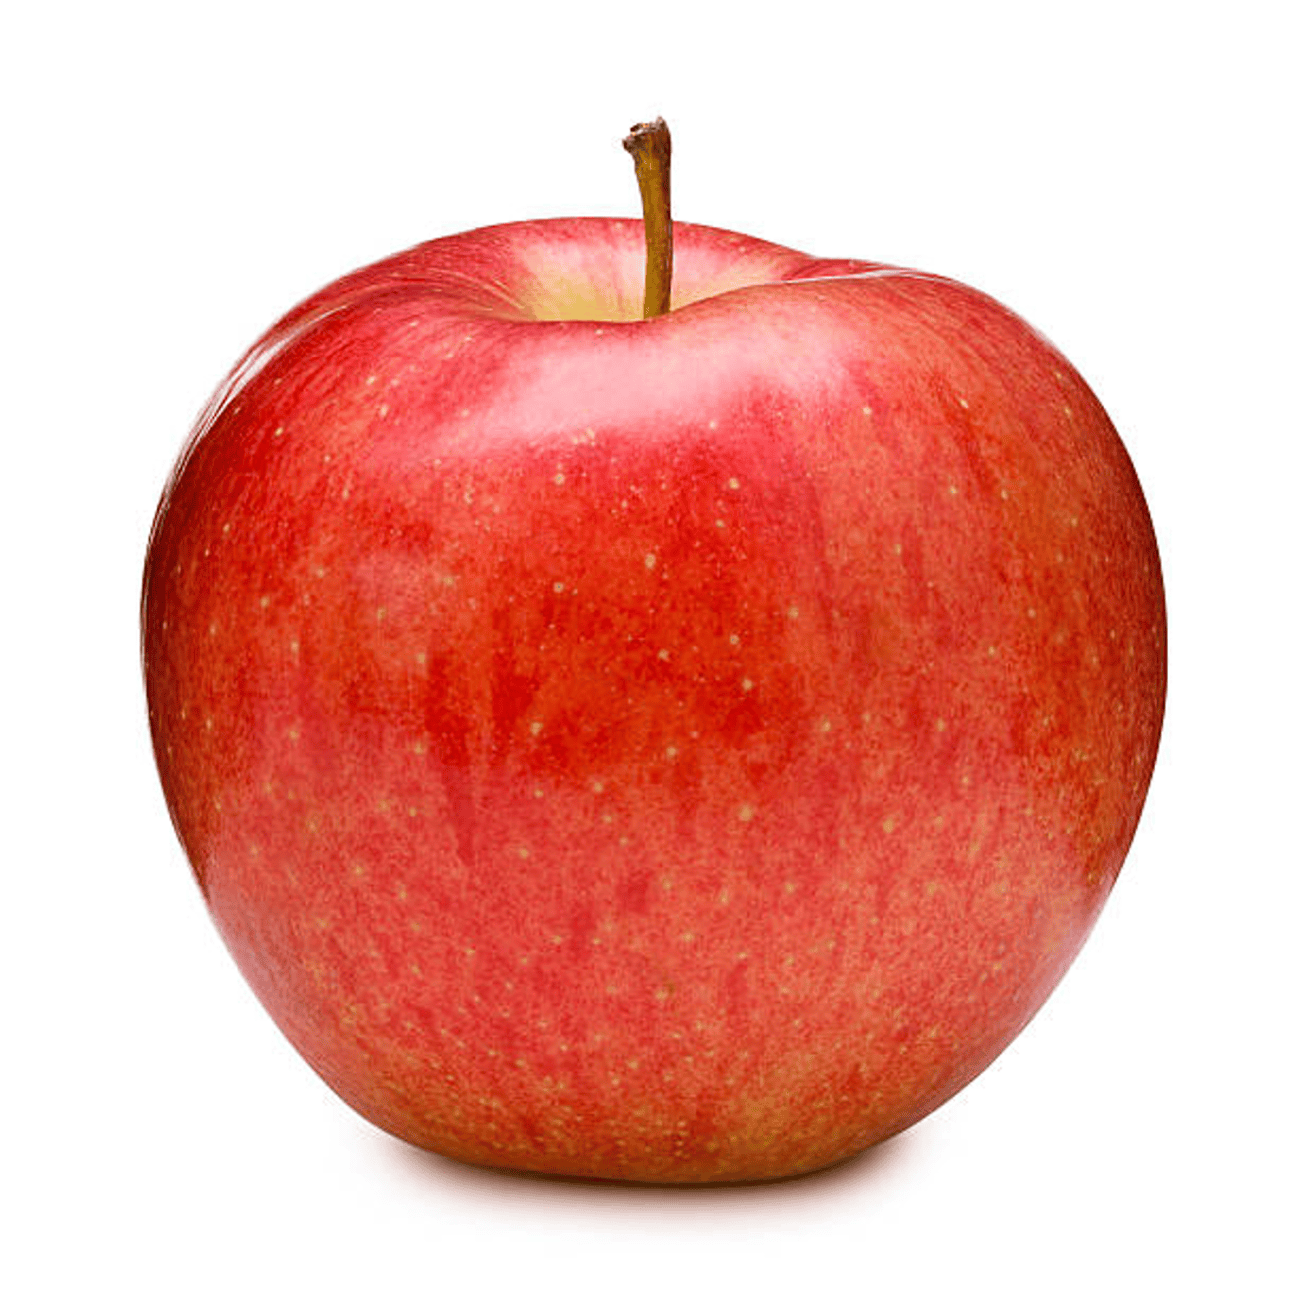
\includegraphics[height = 1cm, width = 1cm]{C8M18 - DT - Q9i.png}}  \adjustbox{scale=\scalefactor}{
\includegraphics[height = 1cm, width = 1cm]{C8M18 - DT - Q9ii.png}}  \adjustbox{scale=\scalefactor}{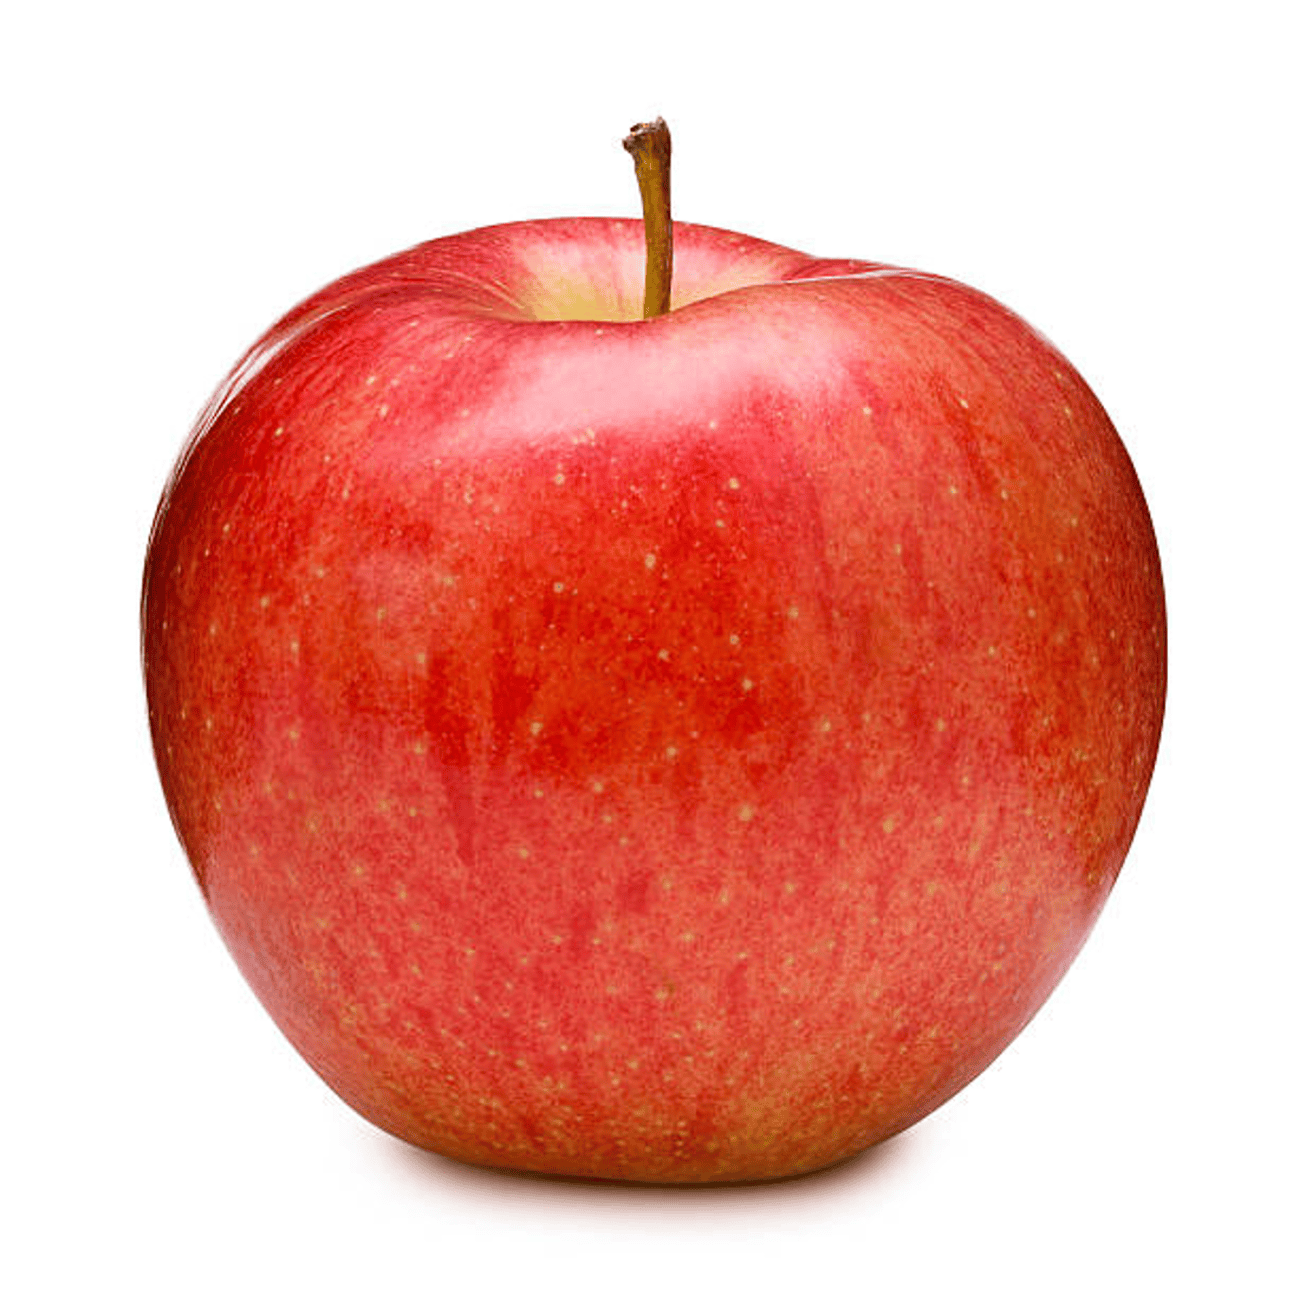
\includegraphics[height = 1cm, width = 1cm]{C8M18 - DT - Q9i.png}} \adjustbox{scale=\scalefactor}{
\includegraphics[height = 1cm, width = 1cm]{C8M18 - DT - Q9ii.png}} \adjustbox{scale=\scalefactor}{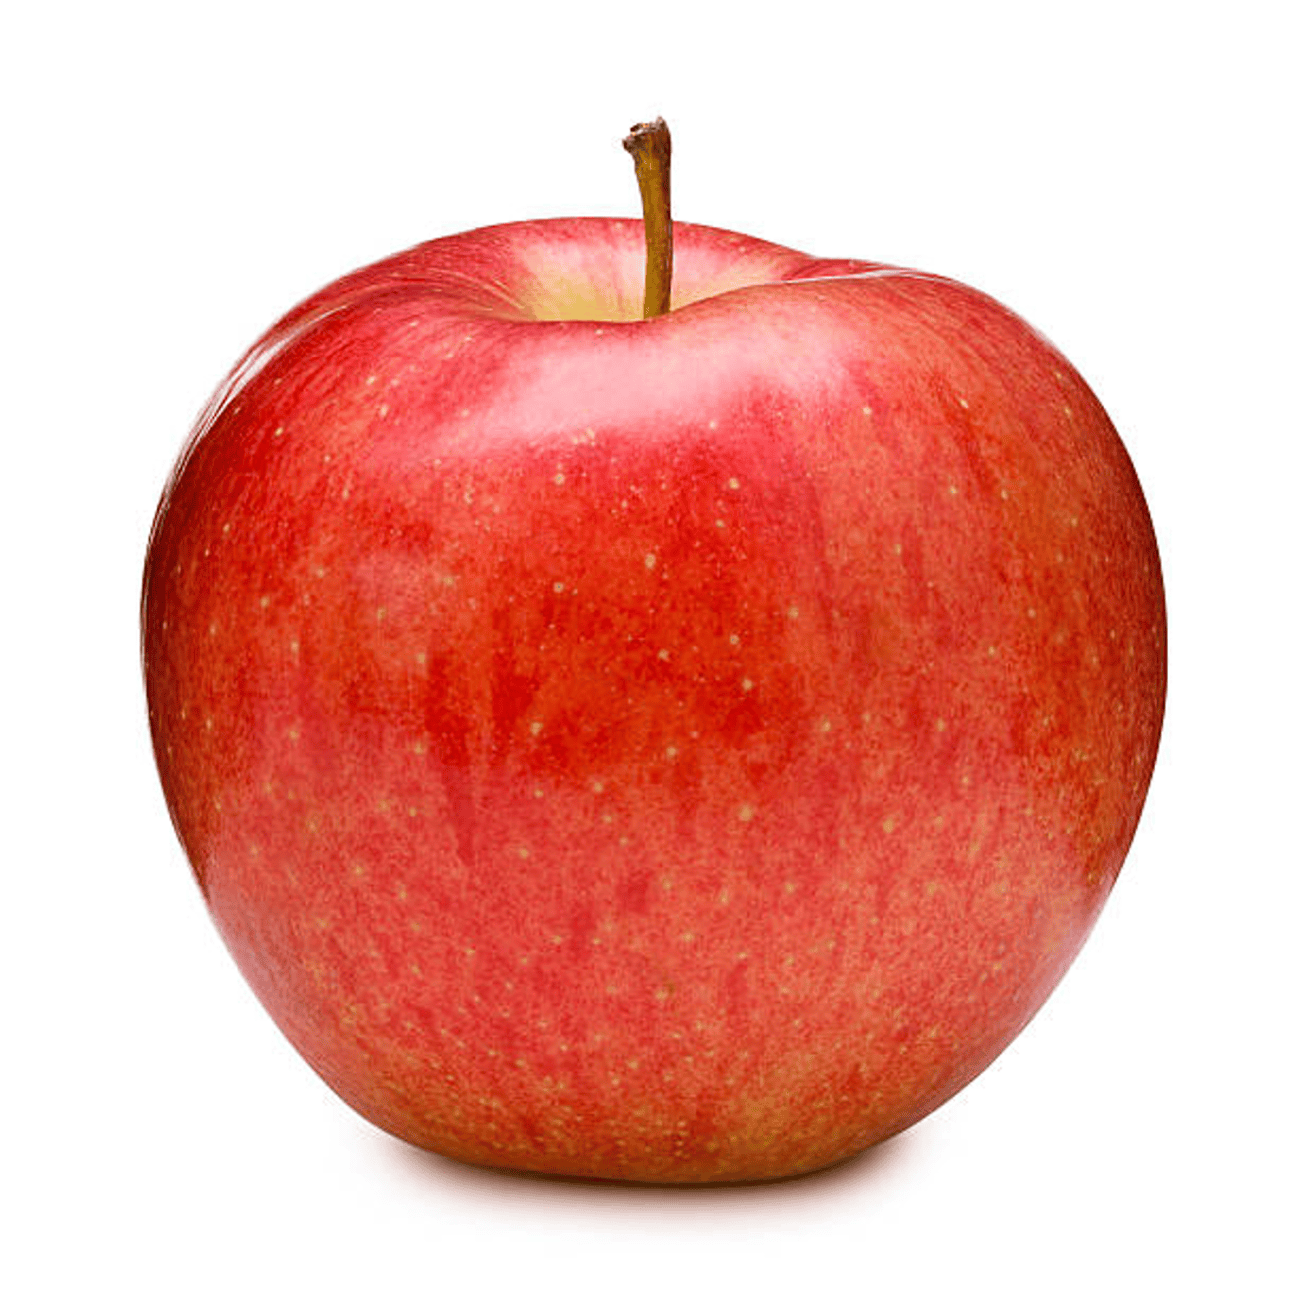
\includegraphics[height = 1cm, width = 1cm]{C8M18 - DT - Q9i.png}} \adjustbox{scale=\scalefactor}{
\includegraphics[height = 1cm, width = 1cm]{C8M18 - DT - Q9ii.png}} \adjustbox{scale=\scalefactor}{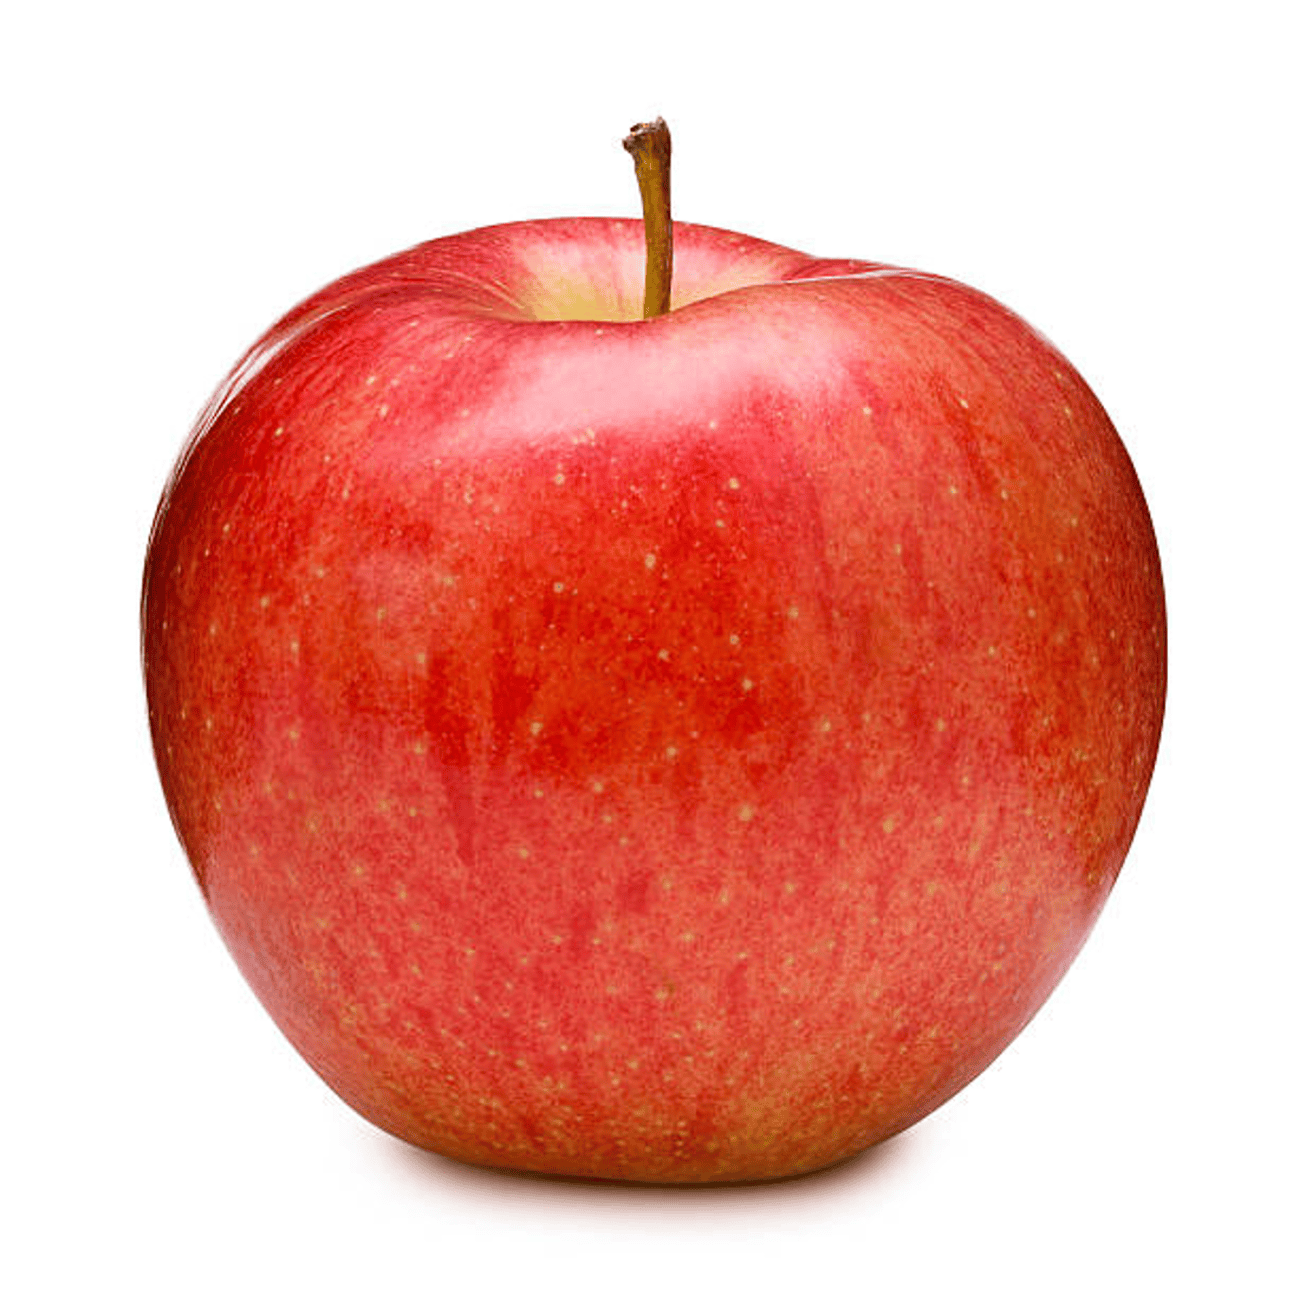
\includegraphics[height = 1cm, width = 1cm]{C8M18 - DT - Q9i.png}}},
optionA={ {{$\dfrac{3}{4}$}}},
optionB={{{$\dfrac{4}{3}$}}},
optionC={{{$\dfrac{4}{7}$}}},
optionD={{{$\dfrac{3}{7}$}}},
correctoption={C},
}

\begin{minipage}{\linewidth}
\hspace{1cm}
\centering
\tiny
\renewcommand{\arraystretch}{1.25}
\begin{tabular}{|M{1.2cm}|M{0.8cm}|M{0.8cm}|M{0.8cm}|M{0.8cm}|M{0.8cm}|}
\hline
Option & A (\ding{55}) & B (\ding{55}) & \cellcolor{cellgreen} C (\ding{51}) & D (\ding{55}) & E \\ 
\hline
8 A & \highno{0\%} & \highno{38\%} & \highno{62\%} & \highno{0\%} & \highno{0\%} \\ 
 \hline 
8 B & \highno{7\%} & \highno{0\%} & \highgreen{93\%} & \highno{0\%} & \highno{0\%} \\ \hline
\end{tabular}
\end{minipage}

\end{frame}
% \input{4. PPT/6. My Answer/Math/C8/117_C8M - Q37}


\begin{frame}[shrink=0.1,label=QPC8QC8M18 - DT - Q4]{Q42 [4. Data Handling]}
\vspace{-0.2cm}
\mcqimgleftFourOne{
questionnumber={42}, 
questionTag={C8M18 - DT - Q4},
questiontext={Find the fruit which is the second least liked by the people.},
imgtabletikz = { {\adjustbox{scale=\scalefactor}{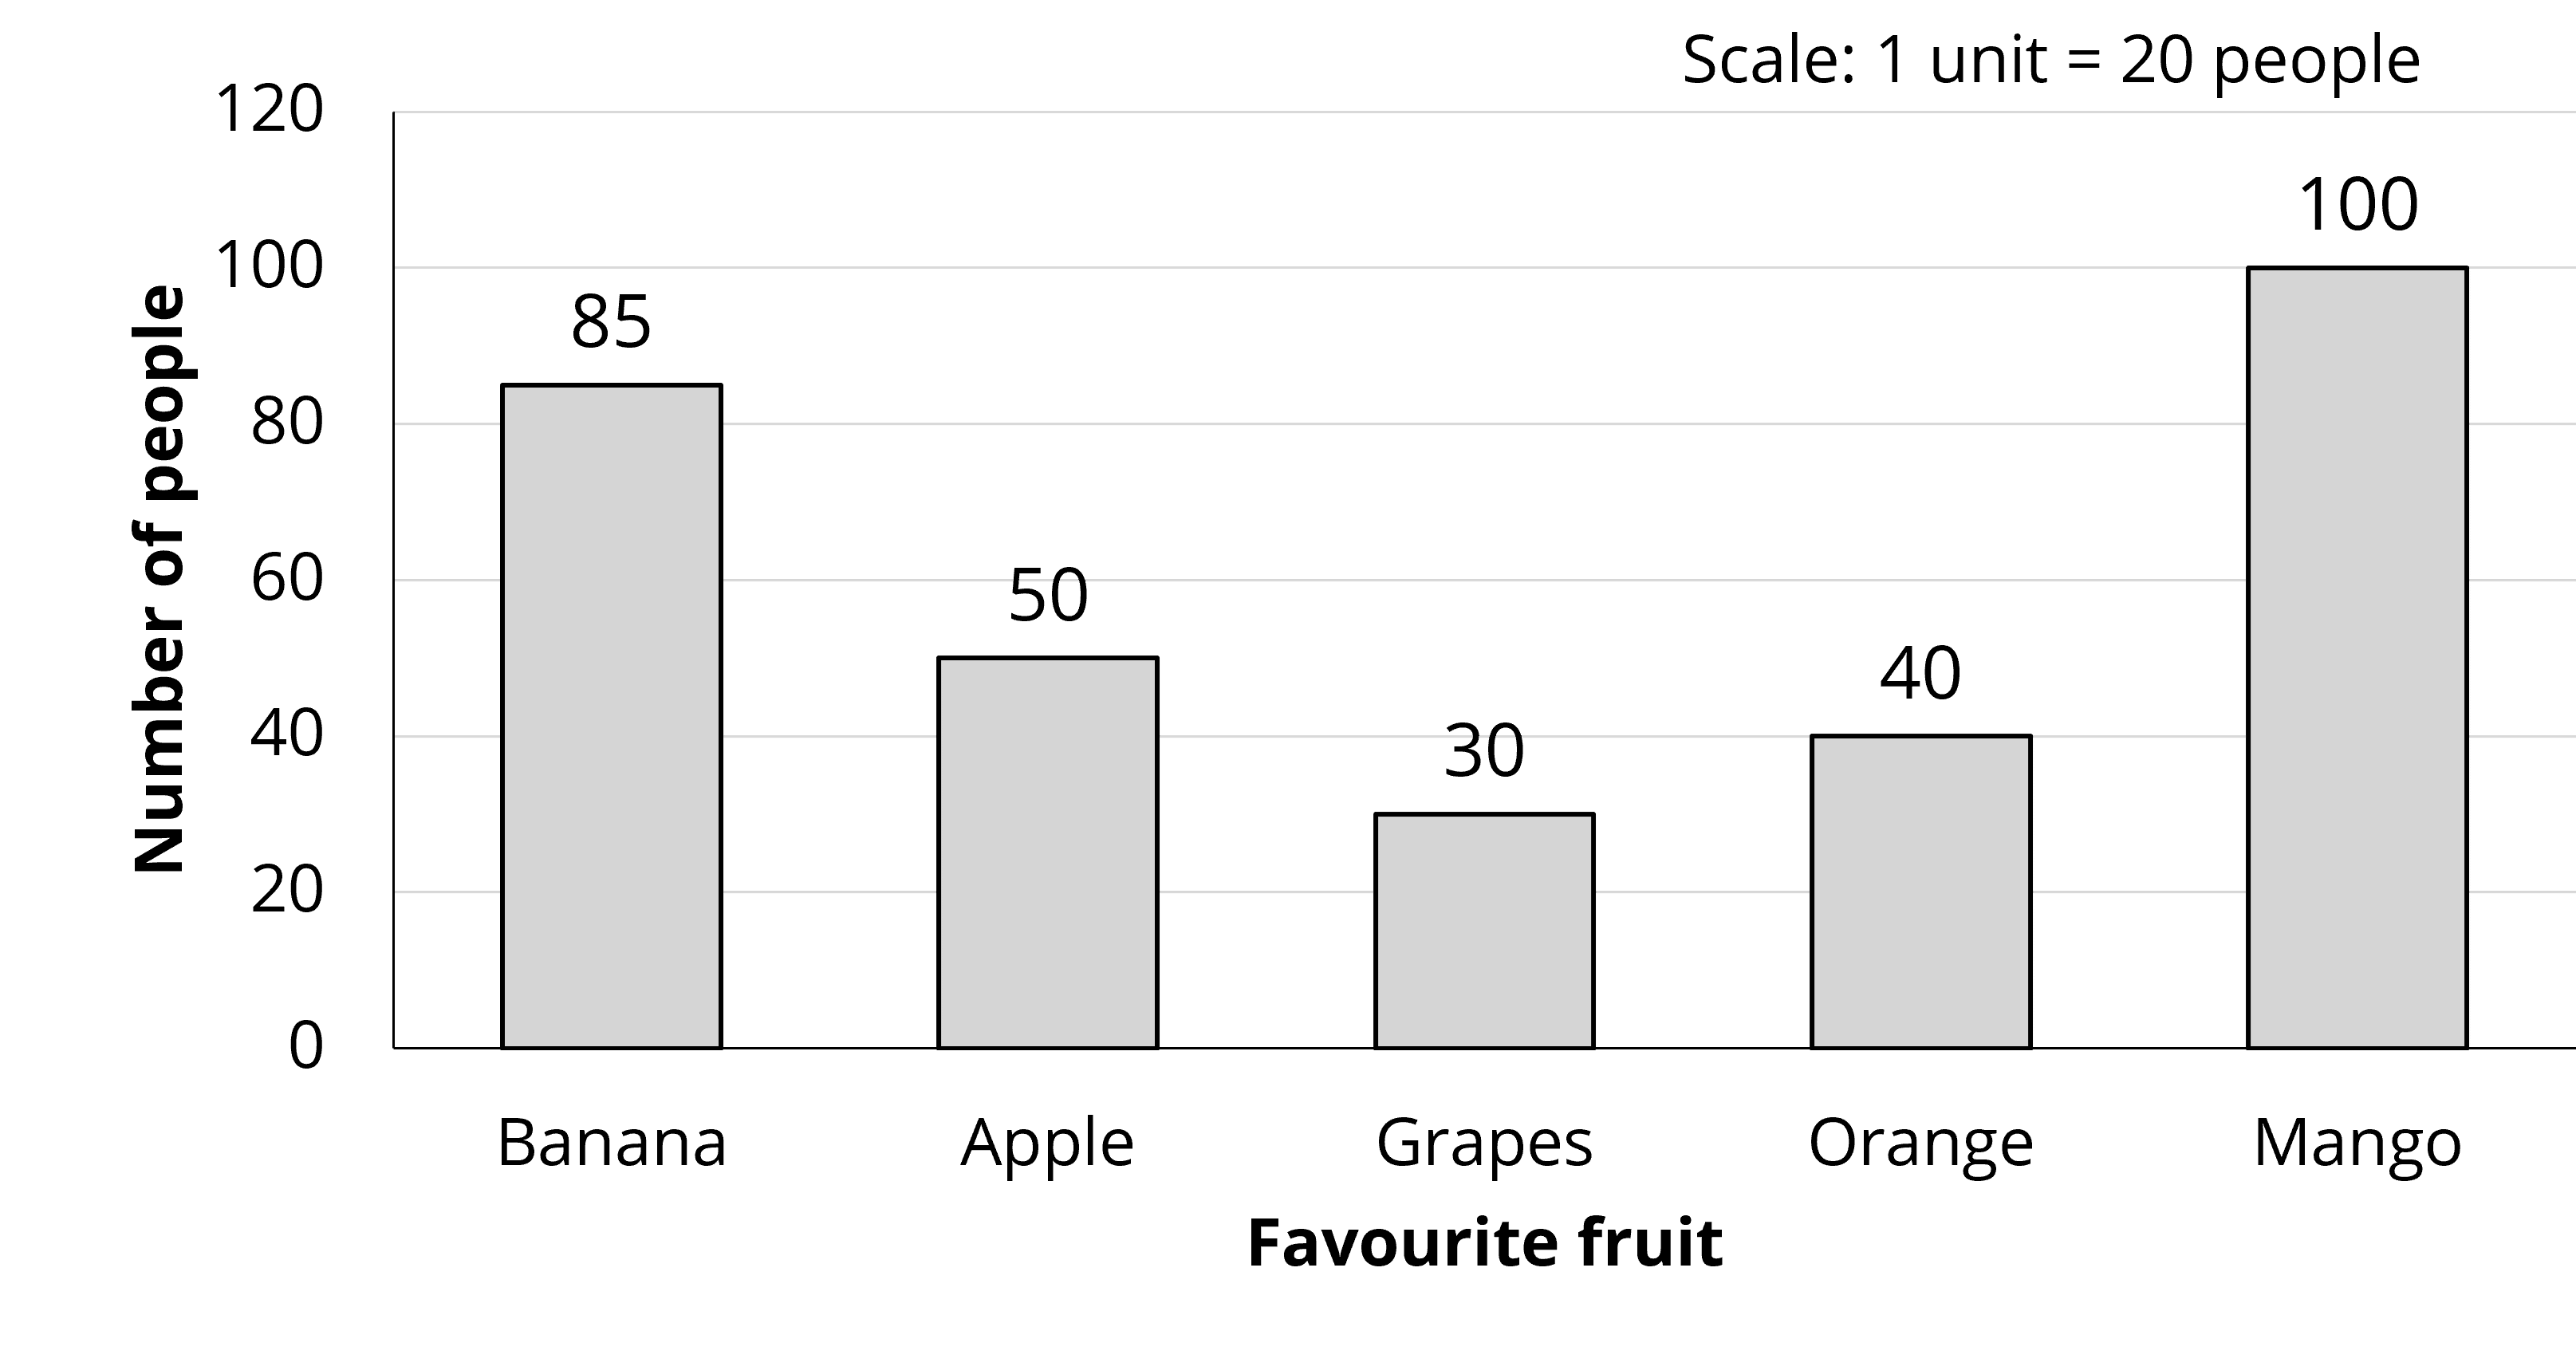
\includegraphics[width=12cm,height=6cm]{C8M18 - DT - Q4.png}}} },
optionA={Grapes },
optionB={Orange },
optionC={Apple and banana},
optionD={Banana},
correctoption={B},
leftmini={0.65},
rightmini={0.25},
}

\begin{minipage}{\linewidth}
\hspace{1cm}
\centering
\tiny
\renewcommand{\arraystretch}{1.25}
\begin{tabular}{|M{1.2cm}|M{0.8cm}|M{0.8cm}|M{0.8cm}|M{0.8cm}|M{0.8cm}|}
\hline
Option & A (\ding{55}) & \cellcolor{cellgreen} B (\ding{51}) & C (\ding{55}) & D (\ding{55}) & E \\ 
\hline
8 A & \highno{8\%} & \highno{46\%} & \highno{0\%} & \highno{46\%} & \highno{0\%} \\ 
 \hline 
8 B & \highno{0\%} & \highgreen{87\%} & \highno{7\%} & \highno{7\%} & \highno{0\%} \\ \hline
\end{tabular}
\end{minipage}

\end{frame}
% \input{4. PPT/6. My Answer/Math/C8/117_C8M - Q42}


\begin{frame}[shrink=0.1,label=QPC8QC8M03 - DT - Q5]{Q25 [5. Squares and Square Roots]}
\vspace{-0.2cm}
\mcqimgleftFourOne{
questionnumber={25}, 
questionTag={C8M03 - DT - Q5},
questiontext={Finding square root by the division method is given below. Find the circled number.},
imgtabletikz={
\renewcommand{\arraystretch}{1.25}
\begin{tabular}{p{0.5cm}|p{0.5cm}p{1cm}}
\multicolumn{2}{c}{} & 12 \\
\cline{2-3}
1& &144 \\
& (-) & 1 \\
\cline{2-3}
{\large{\textcircled{?}}} && \hspace{0.15cm} 44 \\
& (-) & \hspace{0.15cm} 44 \\
\cline{2-3}
&& \hspace{0.3cm} 0\\
\end{tabular}
},
optionA={24},
optionB={22},
optionC={2},
optionD={12},
correctoption={B},
leftmini={0.5},
rightmini={0.4},
}

\begin{minipage}{\linewidth}
\hspace{1cm}
\centering
\tiny
\renewcommand{\arraystretch}{1.25}
\begin{tabular}{|M{1.2cm}|M{0.8cm}|M{0.8cm}|M{0.8cm}|M{0.8cm}|M{0.8cm}|}
\hline
Option & A (\ding{55}) & \cellcolor{cellgreen} B (\ding{51}) & C (\ding{55}) & D (\ding{55}) & E \\ 
\hline
8 A & \highno{15\%} & \highred{38\%} & \highno{31\%} & \highno{15\%} & \highno{0\%} \\ 
 \hline 
8 B & \highno{7\%} & \highno{73\%} & \highno{20\%} & \highno{0\%} & \highno{0\%} \\ \hline
\end{tabular}
\end{minipage}

\end{frame}
% \input{4. PPT/6. My Answer/Math/C8/117_C8M - Q25}


\begin{frame}[shrink=0.1,label=QPC8QC8M03 - DT - Q8]{Q26 [5. Squares and Square Roots]}
\vspace{-0.2cm}
\mcqtextbottomOneFour{
questionnumber={26},
questionTag={C8M03 - DT - Q8},
questiontext={Find the square root of 289.},
optionA={9},
optionB={16},
optionC={28},
optionD={17},
correctoption={D},
}

\begin{minipage}{\linewidth}
\hspace{1cm}
\centering
\tiny
\renewcommand{\arraystretch}{1.25}
\begin{tabular}{|M{1.2cm}|M{0.8cm}|M{0.8cm}|M{0.8cm}|M{0.8cm}|M{0.8cm}|}
\hline
Option & A (\ding{55}) & B (\ding{55}) & C (\ding{55}) & \cellcolor{cellgreen} D (\ding{51}) & E \\ 
\hline
8 A & \highno{8\%} & \highno{0\%} & \highno{31\%} & \highno{54\%} & \highno{8\%} \\ 
 \hline 
8 B & \highno{7\%} & \highno{7\%} & \highno{0\%} & \highgreen{87\%} & \highno{0\%} \\ \hline
\end{tabular}
\end{minipage}

\end{frame}
% \input{4. PPT/6. My Answer/Math/C8/117_C8M - Q26}


\begin{frame}[shrink=0.1,label=QPC8QC8M03 - DT - Q2]{Q50 [5. Squares and Square Roots]}
\vspace{-0.2cm}
\mcqtextbottomOneFour{
questionnumber={50}, 
questionTag={C8M03 - DT - Q2}, 
questiontext={If a number ends with 3 or 7, its square will always end with \rule{80pt}{0.5pt}.},
optionA={0},
optionB={3},
optionC={7},
optionD={9},
correctoption={D},
}

\begin{minipage}{\linewidth}
\hspace{1cm}
\centering
\tiny
\renewcommand{\arraystretch}{1.25}
\begin{tabular}{|M{1.2cm}|M{0.8cm}|M{0.8cm}|M{0.8cm}|M{0.8cm}|M{0.8cm}|}
\hline
Option & A (\ding{55}) & B (\ding{55}) & C (\ding{55}) & \cellcolor{cellgreen} D (\ding{51}) & E \\ 
\hline
8 A & \highno{15\%} & \highno{15\%} & \highno{23\%} & \highno{46\%} & \highno{0\%} \\ 
 \hline 
8 B & \highno{13\%} & \highno{0\%} & \highno{0\%} & \highgreen{80\%} & \highno{7\%} \\ \hline
\end{tabular}
\end{minipage}

\end{frame}
% \input{4. PPT/6. My Answer/Math/C8/117_C8M - Q50}


\begin{frame}[shrink=0.1,label=QPC8QC8M04 - DT - Q5]{Q30 [6. Cubes and Cube Roots]}
\vspace{-0.2cm}
\mcqtextbottomOneFour{
questionnumber={30}, 
questionTag={C8M04 - DT - Q5}, 
questiontext={Simplify: $\sqrt[2]{\sqrt[3]{64}}$ },
optionA={4},
optionB={16},
optionC={2},
optionD={64},
correctoption={C},
}

\begin{minipage}{\linewidth}
\hspace{1cm}
\centering
\tiny
\renewcommand{\arraystretch}{1.25}
\begin{tabular}{|M{1.2cm}|M{0.8cm}|M{0.8cm}|M{0.8cm}|M{0.8cm}|M{0.8cm}|}
\hline
Option & A (\ding{55}) & B (\ding{55}) & \cellcolor{cellgreen} C (\ding{51}) & D (\ding{55}) & E \\ 
\hline
8 A & \highno{15\%} & \highno{54\%} & \highred{8\%} & \highno{0\%} & \highno{23\%} \\ 
 \hline 
8 B & \highno{7\%} & \highno{7\%} & \highgreen{80\%} & \highno{7\%} & \highno{0\%} \\ \hline
\end{tabular}
\end{minipage}

\end{frame}
% \input{4. PPT/6. My Answer/Math/C8/117_C8M - Q30}


\begin{frame}[shrink=0.1,label=QPC8QC8M04 - DT - Q3]{Q33 [6. Cubes and Cube Roots]}
\vspace{-0.2cm}
\mcqtextbottomOneFour{
questionnumber={33}, 
questionTag={C8M04 - DT - Q3}, 
questiontext={Pick the perfect cube from the following.},
optionA={728},
optionB={215},
optionC={343},
optionD={511},
correctoption={C},
}

\begin{minipage}{\linewidth}
\hspace{1cm}
\centering
\tiny
\renewcommand{\arraystretch}{1.25}
\begin{tabular}{|M{1.2cm}|M{0.8cm}|M{0.8cm}|M{0.8cm}|M{0.8cm}|M{0.8cm}|}
\hline
Option & A (\ding{55}) & B (\ding{55}) & \cellcolor{cellgreen} C (\ding{51}) & D (\ding{55}) & E \\ 
\hline
8 A & \highno{23\%} & \highno{54\%} & \highred{23\%} & \highno{0\%} & \highno{0\%} \\ 
 \hline 
8 B & \highno{13\%} & \highno{7\%} & \highno{60\%} & \highno{7\%} & \highno{13\%} \\ \hline
\end{tabular}
\end{minipage}

\end{frame}
% \input{4. PPT/6. My Answer/Math/C8/117_C8M - Q33}


\begin{frame}[shrink=0.1,label=QPC8QC8M04 - DT - Q2]{Q54 [6. Cubes and Cube Roots]}
\vspace{-0.2cm}
\mcqtextbottomOneFour{
questionnumber={54}, 
questionTag={C8M04 - DT - Q2}, 
questiontext={Find the one's digit in the cube of 11.},
optionA={0},
optionB={1},
optionC={2},
optionD={4},
correctoption={B},
}

\begin{minipage}{\linewidth}
\hspace{1cm}
\centering
\tiny
\renewcommand{\arraystretch}{1.25}
\begin{tabular}{|M{1.2cm}|M{0.8cm}|M{0.8cm}|M{0.8cm}|M{0.8cm}|M{0.8cm}|}
\hline
Option & A (\ding{55}) & \cellcolor{cellgreen} B (\ding{51}) & C (\ding{55}) & D (\ding{55}) & E \\ 
\hline
8 A & \highno{15\%} & \highno{54\%} & \highno{15\%} & \highno{8\%} & \highno{8\%} \\ 
 \hline 
8 B & \highno{0\%} & \highgreen{93\%} & \highno{7\%} & \highno{0\%} & \highno{0\%} \\ \hline
\end{tabular}
\end{minipage}

\end{frame}
% \input{4. PPT/6. My Answer/Math/C8/117_C8M - Q54}


\begin{frame}[shrink=0.1,label=QPC8QC8M10 - DT - Q4]{Q21 [7. Comparing Quantities]}
\vspace{-0.2cm}
\mcqtextbottomOneFour{
questionnumber={21}, 
questionTag={C8M10 - DT - Q4}, 
questiontext={In a school's cultural program, 25 students participated in yoga out of 200 students. What percentage of students participated in yoga?},
optionA={12\%},
optionB={12.5\%},
optionC={10\%},
optionD={25\%},
correctoption={B},
}

\begin{minipage}{\linewidth}
\hspace{1cm}
\centering
\tiny
\renewcommand{\arraystretch}{1.25}
\begin{tabular}{|M{1.2cm}|M{0.8cm}|M{0.8cm}|M{0.8cm}|M{0.8cm}|M{0.8cm}|}
\hline
Option & A (\ding{55}) & \cellcolor{cellgreen} B (\ding{51}) & C (\ding{55}) & D (\ding{55}) & E \\ 
\hline
8 A & \highno{0\%} & \highno{54\%} & \highno{8\%} & \highno{31\%} & \highno{8\%} \\ 
 \hline 
8 B & \highno{0\%} & \highgreen{93\%} & \highno{0\%} & \highno{7\%} & \highno{0\%} \\ \hline
\end{tabular}
\end{minipage}

\end{frame}
% \input{4. PPT/6. My Answer/Math/C8/117_C8M - Q21}


\begin{frame}[shrink=0.1,label=QPC8QC8M10 - DT - Q5]{Q43 [7. Comparing Quantities]}
\vspace{-0.2cm}
\mcqtextbottomOneFour{
questionnumber={43}, 
questionTag={C8M10 - DT - Q5}, 
questiontext={Sheela bought a pen for Rs. 100 and sold it for Rs. 115. Then it is \rule{30pt}{0.5pt}.},
optionA={Rs. 255 profit},
optionB={Rs. 15 loss},
optionC={Rs. 15 profit},
optionD={Rs. 5 loss},
correctoption={C},
}

\begin{minipage}{\linewidth}
\hspace{1cm}
\centering
\tiny
\renewcommand{\arraystretch}{1.25}
\begin{tabular}{|M{1.2cm}|M{0.8cm}|M{0.8cm}|M{0.8cm}|M{0.8cm}|M{0.8cm}|}
\hline
Option & A (\ding{55}) & B (\ding{55}) & \cellcolor{cellgreen} C (\ding{51}) & D (\ding{55}) & E \\ 
\hline
8 A & \highno{8\%} & \highno{0\%} & \highgreen{85\%} & \highno{8\%} & \highno{0\%} \\ 
 \hline 
8 B & \highno{0\%} & \highno{7\%} & \highgreen{93\%} & \highno{0\%} & \highno{0\%} \\ \hline
\end{tabular}
\end{minipage}

\end{frame}
% \input{4. PPT/6. My Answer/Math/C8/117_C8M - Q43}


\begin{frame}[shrink=0.1,label=QPC8QC8M10 - DT - Q9]{Q49 [7. Comparing Quantities]}
\vspace{-0.2cm}
\mcqtextbottomOneFour{
questionnumber={49}, 
questionTag={C8M10 - DT - Q9}, 
questiontext={Viyaan's mother deposits Rs. 10,000 in a savings account that offers an interest rate of 3\% compounded annually. How much will she have in her account at the end of the two years?},
optionA={Rs. 10,000},
optionB={Rs. 10,004},
optionC={Rs. 10,609},
optionD={Rs. 10,605},
correctoption={C},
}

\begin{minipage}{\linewidth}
\hspace{1cm}
\centering
\tiny
\renewcommand{\arraystretch}{1.25}
\begin{tabular}{|M{1.2cm}|M{0.8cm}|M{0.8cm}|M{0.8cm}|M{0.8cm}|M{0.8cm}|}
\hline
Option & A (\ding{55}) & B (\ding{55}) & \cellcolor{cellgreen} C (\ding{51}) & D (\ding{55}) & E \\ 
\hline
8 A & \highno{8\%} & \highno{15\%} & \highred{38\%} & \highno{23\%} & \highno{15\%} \\ 
 \hline 
8 B & \highno{0\%} & \highno{0\%} & \highgreen{87\%} & \highno{7\%} & \highno{7\%} \\ \hline
\end{tabular}
\end{minipage}

\end{frame}
% \input{4. PPT/6. My Answer/Math/C8/117_C8M - Q49}


\begin{frame}[shrink=0.1,label=QPC8QC8M10 - DT - Q8]{Q51 [7. Comparing Quantities]}
\vspace{-0.2cm}
\mcqtextbottomOneFour{
questionnumber={51}, 
questionTag={C8M10 - DT - Q8}, 
questiontext={The amount payable is Rs. 106 if the principal is Rs. 100 and the rate is 2\% per annum. Find the number of years. (Hint: Use simple interest)},
optionA={2 years},
optionB={3 years},
optionC={1 year},
optionD={1.5 years},
correctoption={B},
}

\begin{minipage}{\linewidth}
\hspace{1cm}
\centering
\tiny
\renewcommand{\arraystretch}{1.25}
\begin{tabular}{|M{1.2cm}|M{0.8cm}|M{0.8cm}|M{0.8cm}|M{0.8cm}|M{0.8cm}|}
\hline
Option & A (\ding{55}) & \cellcolor{cellgreen} B (\ding{51}) & C (\ding{55}) & D (\ding{55}) & E \\ 
\hline
8 A & \highno{8\%} & \highred{38\%} & \highno{23\%} & \highno{31\%} & \highno{0\%} \\ 
 \hline 
8 B & \highno{7\%} & \highno{73\%} & \highno{20\%} & \highno{0\%} & \highno{0\%} \\ \hline
\end{tabular}
\end{minipage}

\end{frame}
% \input{4. PPT/6. My Answer/Math/C8/117_C8M - Q51}


\begin{frame}[shrink=0.1,label=QPC8QC8M08 - DT - Q5]{Q17 [8. Algebraic Expressions and Identities]}
\vspace{-0.2cm}
\mcqtextbottomOneFour{
questionnumber={17}, 
questionTag={C8M08 - DT - Q5}, 
questiontext={$2a \times b$ is a \rule{80pt}{0.5pt} expression. },
optionA={Trinomial },
optionB={Monomial },
optionC={Binomial },
optionD={Not an expression},
correctoption={B},
}

\begin{minipage}{\linewidth}
\hspace{1cm}
\centering
\tiny
\renewcommand{\arraystretch}{1.25}
\begin{tabular}{|M{1.2cm}|M{0.8cm}|M{0.8cm}|M{0.8cm}|M{0.8cm}|M{0.8cm}|}
\hline
Option & A (\ding{55}) & \cellcolor{cellgreen} B (\ding{51}) & C (\ding{55}) & D (\ding{55}) & E \\ 
\hline
8 A & \highno{15\%} & \highred{23\%} & \highno{38\%} & \highno{15\%} & \highno{8\%} \\ 
 \hline 
8 B & \highno{0\%} & \highno{53\%} & \highno{40\%} & \highno{7\%} & \highno{0\%} \\ \hline
\end{tabular}
\end{minipage}

\end{frame}
% \input{4. PPT/6. My Answer/Math/C8/117_C8M - Q17}


\begin{frame}[shrink=0.1,label=QPC8QC8M08 - DT - Q6]{Q24 [8. Algebraic Expressions and Identities]}
\vspace{-0.2cm}
\mcqtextbottomTwoTwo{
questionnumber={24}, 
questionTag={C8M08 - DT - Q6}, 
questiontext={Find the sum of the given algebraic terms.\\ \hspace{4cm} 		$5x$, $2b$, $2c$, $7x$, $5ab$, $6c$, $9a$	},
optionA={$8x + 2b + 12c + 9a$},
optionB={$12x + 2b + 8c + 9a$},
optionC={$12x + 2b + 8c + 5ab + 9a$},
optionD={$12x + 8c + 16ab$},
correctoption={C},
}

\begin{minipage}{\linewidth}
\hspace{1cm}
\centering
\tiny
\renewcommand{\arraystretch}{1.25}
\begin{tabular}{|M{1.2cm}|M{0.8cm}|M{0.8cm}|M{0.8cm}|M{0.8cm}|M{0.8cm}|}
\hline
Option & A (\ding{55}) & B (\ding{55}) & \cellcolor{cellgreen} C (\ding{51}) & D (\ding{55}) & E \\ 
\hline
8 A & \highno{8\%} & \highno{23\%} & \highno{69\%} & \highno{0\%} & \highno{0\%} \\ 
 \hline 
8 B & \highno{0\%} & \highno{7\%} & \highgreen{87\%} & \highno{0\%} & \highno{7\%} \\ \hline
\end{tabular}
\end{minipage}

\end{frame}
% \input{4. PPT/6. My Answer/Math/C8/117_C8M - Q24}


\begin{frame}[shrink=0.1,label=QPC8QC8M08 - DT - Q9]{Q41 [8. Algebraic Expressions and Identities]}
\vspace{-0.2cm}
\mcqimgleftFourOne{
questionnumber={41}, 
questionTag={C8M08 - DT - Q9},
questiontext={Match the following.},
imgtabletikz = {
\begin{table}[H]
\centering
\renewcommand{\arraystretch}{1.25}
\begin{tabular}{|p{0.5cm}|p{2cm}|p{0.2cm}|p{0.5cm}|p{3cm}|}
\cline{1-5} 
\multicolumn{2}{|c|}{\textbf{Identity }} & 
\multirow{5}{*}{} &   
\multicolumn{2}{c|}{\textbf{Expansion of identity}} \\
\cline{1-2}\cline{4-5} i.  & $(a+b)^2$ &   & a. & $a^2-2ab+b^2$ \\
\cline{1-2}\cline{4-5} ii. & $(a)^2 - (b)^2$ &   & b. &  $a^2+2ab+b^2$ \\
\cline{1-2}\cline{4-5} iii.  & $(a-b)^2$ &   & c. & $(a+b)(a-b)$\\
\hline
\end{tabular}
\end{table}
},
optionA={i - b, ii - c, iii - a},
optionB={i - c, ii - b, iii - a},
optionC={i - a, ii - c, iii - b},
optionD={i - b, ii - a, iii - c},
correctoption={A},
leftmini={0.5},
rightmini={0.3},
}

\begin{minipage}{\linewidth}
\hspace{1cm}
\centering
\tiny
\renewcommand{\arraystretch}{1.25}
\begin{tabular}{|M{1.2cm}|M{0.8cm}|M{0.8cm}|M{0.8cm}|M{0.8cm}|M{0.8cm}|}
\hline
Option & \cellcolor{cellgreen} A (\ding{51}) & B (\ding{55}) & C (\ding{55}) & D (\ding{55}) & E \\ 
\hline
8 A & \highno{46\%} & \highno{54\%} & \highno{0\%} & \highno{0\%} & \highno{0\%} \\ 
 \hline 
8 B & \highno{73\%} & \highno{7\%} & \highno{0\%} & \highno{20\%} & \highno{0\%} \\ \hline
\end{tabular}
\end{minipage}

\end{frame}
% \input{4. PPT/6. My Answer/Math/C8/117_C8M - Q41}


\begin{frame}[shrink=0.1,label=QPC8QC8M08 - DT - Q8]{Q47 [8. Algebraic Expressions and Identities]}
\vspace{-0.2cm}
\mcqtextbottomOneFour{
questionnumber={47}, 
questionTag={C8M08 - DT - Q8}, 
questiontext={Find the area of the rectangular box with the given values. \\ \hspace{4cm} Length = $5a+b$, Breadth = $6y$},
optionA={$30ay + 6yb$},
optionB={$30aby$},
optionC={$18ay + by$},
optionD={$5a+b+6y$},
correctoption={A},
}

\begin{minipage}{\linewidth}
\hspace{1cm}
\centering
\tiny
\renewcommand{\arraystretch}{1.25}
\begin{tabular}{|M{1.2cm}|M{0.8cm}|M{0.8cm}|M{0.8cm}|M{0.8cm}|M{0.8cm}|}
\hline
Option & \cellcolor{cellgreen} A (\ding{51}) & B (\ding{55}) & C (\ding{55}) & D (\ding{55}) & E \\ 
\hline
8 A & \highred{8\%} & \highno{38\%} & \highno{15\%} & \highno{38\%} & \highno{0\%} \\ 
 \hline 
8 B & \highno{53\%} & \highno{40\%} & \highno{7\%} & \highno{0\%} & \highno{0\%} \\ \hline
\end{tabular}
\end{minipage}

\end{frame}
% \input{4. PPT/6. My Answer/Math/C8/117_C8M - Q47}


\begin{frame}[shrink=0.1,label=QPC8QC8M08 - DT - Q10]{Q52 [8. Algebraic Expressions and Identities]}
\vspace{-0.2cm}
\mcqtextbottomTwoTwo{
questionnumber={52}, 
questionTag={C8M08 - DT - Q10}, 
questiontext={Which of the following is incorrect for the value of $x$?},
optionA={ {{$\dfrac{x}{2}$}} $-$ $x^2 + 20 = 6$ is true for $x=4$},
optionB={$7x^3+3x=52$ is true for $x=2$},
optionC={ $x^2+2x+4=19$ is true for $x=3$},
optionD={None of these},
correctoption={B},
}

\begin{minipage}{\linewidth}
\hspace{1cm}
\centering
\tiny
\renewcommand{\arraystretch}{1.25}
\begin{tabular}{|M{1.2cm}|M{0.8cm}|M{0.8cm}|M{0.8cm}|M{0.8cm}|M{0.8cm}|}
\hline
Option & A (\ding{55}) & \cellcolor{cellgreen} B (\ding{51}) & C (\ding{55}) & D (\ding{55}) & E \\ 
\hline
8 A & \highno{38\%} & \highred{23\%} & \highno{8\%} & \highno{23\%} & \highno{8\%} \\ 
 \hline 
8 B & \highno{20\%} & \highno{53\%} & \highno{13\%} & \highno{13\%} & \highno{0\%} \\ \hline
\end{tabular}
\end{minipage}

\end{frame}
% \input{4. PPT/6. My Answer/Math/C8/117_C8M - Q52}


\begin{frame}[shrink=0.1,label=QPC8QC8M17 - DT - Q4]{Q16 [9. Mensuration]}
\vspace{-0.2cm}
\mcqtextbottomOneFour{
questionnumber={16}, 
questionTag={C8M17 - DT - Q4}, 
questiontext={Find the height of the trapezium, if the sum of its parallel sides is 18 cm and the area of the trapezium is 90 $cm^2$.},
optionA={81 cm},
optionB={45 cm },
optionC={5 cm},
optionD={10 cm},
correctoption={D},
}

\begin{minipage}{\linewidth}
\hspace{1cm}
\centering
\tiny
\renewcommand{\arraystretch}{1.25}
\begin{tabular}{|M{1.2cm}|M{0.8cm}|M{0.8cm}|M{0.8cm}|M{0.8cm}|M{0.8cm}|}
\hline
Option & A (\ding{55}) & B (\ding{55}) & C (\ding{55}) & \cellcolor{cellgreen} D (\ding{51}) & E \\ 
\hline
8 A & \highno{31\%} & \highno{23\%} & \highno{15\%} & \highred{15\%} & \highno{15\%} \\ 
 \hline 
8 B & \highno{0\%} & \highno{7\%} & \highno{7\%} & \highgreen{80\%} & \highno{7\%} \\ \hline
\end{tabular}
\end{minipage}

\end{frame}
% \input{4. PPT/6. My Answer/Math/C8/117_C8M - Q16}


\begin{frame}[shrink=0.1,label=QPC8QC8M17 - DT - Q8]{Q39 [9. Mensuration]}
\vspace{-0.2cm}
\mcqtextbottomOneFour{
questionnumber={39}, 
questionTag={C8M17 - DT - Q8}, 
questiontext={How many faces are there on the cuboid's lateral surface?},
optionA={0},
optionB={6},
optionC={8},
optionD={4},
correctoption={D},
}

\begin{minipage}{\linewidth}
\hspace{1cm}
\centering
\tiny
\renewcommand{\arraystretch}{1.25}
\begin{tabular}{|M{1.2cm}|M{0.8cm}|M{0.8cm}|M{0.8cm}|M{0.8cm}|M{0.8cm}|}
\hline
Option & A (\ding{55}) & B (\ding{55}) & C (\ding{55}) & \cellcolor{cellgreen} D (\ding{51}) & E \\ 
\hline
8 A & \highno{15\%} & \highno{31\%} & \highno{31\%} & \highred{15\%} & \highno{8\%} \\ 
 \hline 
8 B & \highno{0\%} & \highno{27\%} & \highno{7\%} & \highno{67\%} & \highno{0\%} \\ \hline
\end{tabular}
\end{minipage}

\end{frame}
% \input{4. PPT/6. My Answer/Math/C8/117_C8M - Q39}


\begin{frame}[shrink=0.1,label=QPC8QC8M17 - DT - Q6]{Q40 [9. Mensuration]}
\vspace{-0.2cm}
\mcqimgleftFourOne{
questionnumber={40}, 
questionTag={C8M17 - DT - Q6}, 
questiontext={The expression used for calculating the volume of a cylinder is \rule{50pt}{0.5pt}.},
imgtabletikz ={
\tikzset{every picture/.style={line width=0.75pt,scale=\scalefactor}} 
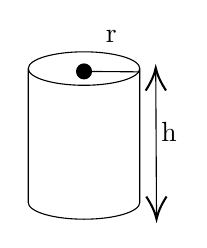
\begin{tikzpicture}[x=0.75pt,y=0.75pt,yscale=-1,xscale=1]
\draw   (262.75,42.42) -- (262.75,106.94) .. controls (262.75,111.39) and (250.72,115) .. (235.88,115) .. controls (221.03,115) and (209,111.39) .. (209,106.94) -- (209,42.42) .. controls (209,37.96) and (221.03,34.35) .. (235.88,34.35) .. controls (250.72,34.35) and (262.75,37.96) .. (262.75,42.42) .. controls (262.75,46.87) and (250.72,50.48) .. (235.88,50.48) .. controls (221.03,50.48) and (209,46.87) .. (209,42.42) ;
\draw    (270.44,44.08) -- (270.8,113) ;
\draw [shift={(270.82,115)}, rotate = 269.7] [color={rgb, 255:red, 0; green, 0; blue, 0 }  ][line width=0.75]    (10.93,-4.9) .. controls (6.95,-2.3) and (3.31,-0.67) .. (0,0) .. controls (3.31,0.67) and (6.95,2.3) .. (10.93,4.9)   ;
\draw [shift={(270.43,42.08)}, rotate = 89.7] [color={rgb, 255:red, 0; green, 0; blue, 0 }  ][line width=0.75]    (10.93,-4.9) .. controls (6.95,-2.3) and (3.31,-0.67) .. (0,0) .. controls (3.31,0.67) and (6.95,2.3) .. (10.93,4.9)   ;
\draw    (235.88,43.79) -- (262.75,44.01) ;
\draw [shift={(235.88,43.79)}, rotate = 0.46] [color={rgb, 255:red, 0; green, 0; blue, 0 }  ][fill={rgb, 255:red, 0; green, 0; blue, 0 }  ][line width=0.75]      (0, 0) circle [x radius= 3.35, y radius= 3.35]   ;
\draw (271.84,67.03) node [anchor=north west][inner sep=0.75pt]   [align=left] {h};
\draw (245.09,22.99) node [anchor=north west][inner sep=0.75pt]   [align=left] {r};
\end{tikzpicture}   },
optionA={$2\pi r(r + h)$ cu. units},
optionB={$2\pi rh$ cu. units},
optionC={$\pi r^2h$ cu. units},
optionD={$\pi r^2$ cu. units},
correctoption={C},
leftmini={0.5},
rightmini={0.4},}

\begin{minipage}{\linewidth}
\hspace{1cm}
\centering
\tiny
\renewcommand{\arraystretch}{1.25}
\begin{tabular}{|M{1.2cm}|M{0.8cm}|M{0.8cm}|M{0.8cm}|M{0.8cm}|M{0.8cm}|}
\hline
Option & A (\ding{55}) & B (\ding{55}) & \cellcolor{cellgreen} C (\ding{51}) & D (\ding{55}) & E \\ 
\hline
8 A & \highno{38\%} & \highno{15\%} & \highred{15\%} & \highno{8\%} & \highno{23\%} \\ 
 \hline 
8 B & \highno{7\%} & \highno{13\%} & \highgreen{80\%} & \highno{0\%} & \highno{0\%} \\ \hline
\end{tabular}
\end{minipage}

\end{frame}
% \input{4. PPT/6. My Answer/Math/C8/117_C8M - Q40}


\begin{frame}[shrink=0.1,label=QPC8QC8M17 - CT - Q1]{Q58 [9. Mensuration]}
\vspace{-0.2cm}
\mcqtextbottomOneFour{
questionnumber={58 - Critical Thinking},
questionTag = {C8M17 - CT - Q1},
questiontext = {Varun had 25 cubes of sides 3 cm each. Varun needs to send the cubes in the parcel in the box of dimensions 12 cm $\times$ 9 cm $\times$ 6 cm. How many cubes are left outside the box?},
optionA={1},
optionB={24},
optionC={13},
optionD={21},
correctoption = {A},
}

\begin{minipage}{\linewidth}
\hspace{1cm}
\centering
\tiny
\renewcommand{\arraystretch}{1.25}
\begin{tabular}{|M{1.2cm}|M{0.8cm}|M{0.8cm}|M{0.8cm}|M{0.8cm}|M{0.8cm}|}
\hline
Option & \cellcolor{cellgreen} A (\ding{51}) & B (\ding{55}) & C (\ding{55}) & D (\ding{55}) & E \\ 
\hline
8 A & \highred{15\%} & \highno{54\%} & \highno{8\%} & \highno{15\%} & \highno{8\%} \\ 
 \hline 
8 B & \highred{20\%} & \highno{13\%} & \highno{53\%} & \highno{0\%} & \highno{13\%} \\ \hline
\end{tabular}
\end{minipage}

\end{frame}
% \input{4. PPT/6. My Answer/Math/C8/117_C8M - Q58 - Critical Thinking}


\begin{frame}[shrink=0.1,label=QPC8QC8M02 - DT - Q2]{Q19 [10. Exponents and Powers]}
\vspace{-0.2cm}
\mcqtextbottomOneFour{
questionnumber={19}, 
questionTag={C8M02 - DT - Q2}, 
questiontext={$10^{-2} \times 2^2$ is similar to \rule{40pt}{0.5pt}. },
optionA={ {{$\dfrac{1}{10^{-2}}$}} $\times$ 4},
optionB={ {{$\dfrac{1}{10^{2}}$}} $\times$ 4},
optionC={ {{$\dfrac{1}{1000}$}} $\times$ 2},
optionD={100 $\times$ 4},
correctoption={B},
}

\begin{minipage}{\linewidth}
\hspace{1cm}
\centering
\tiny
\renewcommand{\arraystretch}{1.25}
\begin{tabular}{|M{1.2cm}|M{0.8cm}|M{0.8cm}|M{0.8cm}|M{0.8cm}|M{0.8cm}|}
\hline
Option & A (\ding{55}) & \cellcolor{cellgreen} B (\ding{51}) & C (\ding{55}) & D (\ding{55}) & E \\ 
\hline
8 A & \highno{23\%} & \highno{46\%} & \highno{8\%} & \highno{23\%} & \highno{0\%} \\ 
 \hline 
8 B & \highno{0\%} & \highgreen{93\%} & \highno{7\%} & \highno{0\%} & \highno{0\%} \\ \hline
\end{tabular}
\end{minipage}

\end{frame}
% \input{4. PPT/6. My Answer/Math/C8/117_C8M - Q19}


\begin{frame}[shrink=0.1,label=QPC8QC8M02 - DT - Q8]{Q32 [10. Exponents and Powers]}
\vspace{-0.2cm}
\mcqtextbottomOneFour{
questionnumber={32}, 
questionTag={C8M02 - DT - Q8}, 
questiontext={The cost of 10 kg of fig is Rs. 2.4 $\times$ 10$^3$ and the cost of 1 kg of red apple is Rs. 1.2 $\times$ 10$^2$ . Find the total cost.},
optionA={Rs. 2.412 $\times$ $10^3$},
optionB={Rs. 2.52 $\times$ $10^3$},
optionC={Rs. 25.2$\times$ $10^3$ },
optionD={Rs. 2.512$\times$ $10^2$},
correctoption={B},
}

\begin{minipage}{\linewidth}
\hspace{1cm}
\centering
\tiny
\renewcommand{\arraystretch}{1.25}
\begin{tabular}{|M{1.2cm}|M{0.8cm}|M{0.8cm}|M{0.8cm}|M{0.8cm}|M{0.8cm}|}
\hline
Option & A (\ding{55}) & \cellcolor{cellgreen} B (\ding{51}) & C (\ding{55}) & D (\ding{55}) & E \\ 
\hline
8 A & \highno{54\%} & \highred{8\%} & \highno{23\%} & \highno{0\%} & \highno{15\%} \\ 
 \hline 
8 B & \highno{7\%} & \highno{67\%} & \highno{7\%} & \highno{0\%} & \highno{20\%} \\ \hline
\end{tabular}
\end{minipage}

\end{frame}
% \input{4. PPT/6. My Answer/Math/C8/117_C8M - Q32}


\begin{frame}[shrink=0.1,label=QPC8QC8M02 - DT - Q3]{Q34 [10. Exponents and Powers]}
\vspace{-0.2cm}
\mcqtextbottomOneFour{
questionnumber={34}, 
questionTag={C8M02 - DT - Q3}, 
questiontext={Find the product of $a^m$ and its multiplicative inverse.},
optionA={{{$\dfrac{1}{a^m}$}}},
optionB={$a^{-m}$},
optionC={0},
optionD={1},
correctoption={D},
}

\begin{minipage}{\linewidth}
\hspace{1cm}
\centering
\tiny
\renewcommand{\arraystretch}{1.25}
\begin{tabular}{|M{1.2cm}|M{0.8cm}|M{0.8cm}|M{0.8cm}|M{0.8cm}|M{0.8cm}|}
\hline
Option & A (\ding{55}) & B (\ding{55}) & C (\ding{55}) & \cellcolor{cellgreen} D (\ding{51}) & E \\ 
\hline
8 A & \highno{46\%} & \highno{15\%} & \highno{8\%} & \highred{23\%} & \highno{8\%} \\ 
 \hline 
8 B & \highno{40\%} & \highno{7\%} & \highno{0\%} & \highno{53\%} & \highno{0\%} \\ \hline
\end{tabular}
\end{minipage}

\end{frame}
% \input{4. PPT/6. My Answer/Math/C8/117_C8M - Q34}


\begin{frame}[shrink=0.1,label=QPC8QC8M02 - DT - Q10]{Q44 [10. Exponents and Powers]}
\vspace{-0.2cm}
\mcqtextbottomOneFour{
questionnumber={44}, 
questionTag={C8M02 - DT - Q10}, 
questiontext={Find the number greater than 10$^2$},
optionA={10 $\times$ 10$^2$},
optionB={10 $\times$ 10$^{-2}$},
optionC={100 $\times$ 10$^{-2}$},
optionD={10 $\times$ 10$^{-5}$},
correctoption={A},
}

\begin{minipage}{\linewidth}
\hspace{1cm}
\centering
\tiny
\renewcommand{\arraystretch}{1.25}
\begin{tabular}{|M{1.2cm}|M{0.8cm}|M{0.8cm}|M{0.8cm}|M{0.8cm}|M{0.8cm}|}
\hline
Option & \cellcolor{cellgreen} A (\ding{51}) & B (\ding{55}) & C (\ding{55}) & D (\ding{55}) & E \\ 
\hline
8 A & \highno{46\%} & \highno{15\%} & \highno{15\%} & \highno{23\%} & \highno{0\%} \\ 
 \hline 
8 B & \highgreen{87\%} & \highno{0\%} & \highno{0\%} & \highno{7\%} & \highno{7\%} \\ \hline
\end{tabular}
\end{minipage}

\end{frame}
% \input{4. PPT/6. My Answer/Math/C8/117_C8M - Q44}


\begin{frame}[shrink=0.1,label=QPC8QC8M02 - DT - Q5]{Q48 [10. Exponents and Powers]}
\vspace{-0.2cm}
\mcqtextbottomOneFour{
questionnumber={48}, 
questionTag={C8M02 - DT - Q5}, 
questiontext={Find the wrong one.},
optionA={$a^m \divisionsymbol b^m = {\large{(\frac{a}{b})}}^m$},
optionB={$a^m \times b^m = (ab)^m$},
optionC={$a^m \divisionsymbol a^n = (a)^{m \divisionsymbol n}$},
optionD={$a^m \times a^n = (a)^{m+n}$},
correctoption={C},
}

\begin{minipage}{\linewidth}
\hspace{1cm}
\centering
\tiny
\renewcommand{\arraystretch}{1.25}
\begin{tabular}{|M{1.2cm}|M{0.8cm}|M{0.8cm}|M{0.8cm}|M{0.8cm}|M{0.8cm}|}
\hline
Option & A (\ding{55}) & B (\ding{55}) & \cellcolor{cellgreen} C (\ding{51}) & D (\ding{55}) & E \\ 
\hline
8 A & \highno{8\%} & \highno{23\%} & \highno{69\%} & \highno{0\%} & \highno{0\%} \\ 
 \hline 
8 B & \highno{0\%} & \highno{0\%} & \highgreen{100\%} & \highno{0\%} & \highno{0\%} \\ \hline
\end{tabular}
\end{minipage}

\end{frame}
% \input{4. PPT/6. My Answer/Math/C8/117_C8M - Q48}


\begin{frame}[shrink=0.1,label=QPC8QC8M11 - DT - Q5]{Q14 [11. Direct and Inverse Proportions]}
\vspace{-0.2cm}
\mcqtextbottomOneFour{
questionnumber={14}, 
questionTag={C8M11 - DT - Q5}, 
questiontext={When global warming increases, the temperature increases, and rainfall decreases. Identify the factor that is inversely proportional to global warming.},
optionA={Global warming},
optionB={Temperature },
optionC={Rainfall},
optionD={Ozone},
correctoption={C},
}

\begin{minipage}{\linewidth}
\hspace{1cm}
\centering
\tiny
\renewcommand{\arraystretch}{1.25}
\begin{tabular}{|M{1.2cm}|M{0.8cm}|M{0.8cm}|M{0.8cm}|M{0.8cm}|M{0.8cm}|}
\hline
Option & A (\ding{55}) & B (\ding{55}) & \cellcolor{cellgreen} C (\ding{51}) & D (\ding{55}) & E \\ 
\hline
8 A & \highno{23\%} & \highno{15\%} & \highred{15\%} & \highno{38\%} & \highno{8\%} \\ 
 \hline 
8 B & \highno{7\%} & \highno{0\%} & \highgreen{80\%} & \highno{7\%} & \highno{7\%} \\ \hline
\end{tabular}
\end{minipage}

\end{frame}
% \input{4. PPT/6. My Answer/Math/C8/117_C8M - Q14}


\begin{frame}[shrink=0.1,label=QPC8QC8M11 - DT - Q1]{Q15 [11. Direct and Inverse Proportions]}
\vspace{-0.2cm}
\mcqtextbottomOneFour{
questionnumber={15}, 
questionTag={C8M11 - DT - Q1}, 
questiontext={The cost of one piece of cake is Rs. 10. What is the cost of four pieces of cake?},
optionA={Rs. 400},
optionB={Rs. 4},
optionC={Rs. 40},
optionD={Rs. 10},
correctoption={C},
}

\begin{minipage}{\linewidth}
\hspace{1cm}
\centering
\tiny
\renewcommand{\arraystretch}{1.25}
\begin{tabular}{|M{1.2cm}|M{0.8cm}|M{0.8cm}|M{0.8cm}|M{0.8cm}|M{0.8cm}|}
\hline
Option & A (\ding{55}) & B (\ding{55}) & \cellcolor{cellgreen} C (\ding{51}) & D (\ding{55}) & E \\ 
\hline
8 A & \highno{0\%} & \highno{23\%} & \highgreen{77\%} & \highno{0\%} & \highno{0\%} \\ 
 \hline 
8 B & \highno{0\%} & \highno{7\%} & \highgreen{93\%} & \highno{0\%} & \highno{0\%} \\ \hline
\end{tabular}
\end{minipage}

\end{frame}
% \input{4. PPT/6. My Answer/Math/C8/117_C8M - Q15}


\begin{frame}[shrink=0.1,label=QPC8QC8M11 - DT - Q3]{Q27 [11. Direct and Inverse Proportions]}
\vspace{-0.2cm}
\mcqimgleftFourOne{
questionnumber={27}, 
questionTag={C8M11 - DT - Q3}, 
questiontext={Find the missing weight.},
imgtabletikz = { 
\renewcommand{\arraystretch}{1.5}
\begin{tabular}{|p{7cm}|p{3cm}|}
\hline
\adjustbox{scale=\scalefactor}{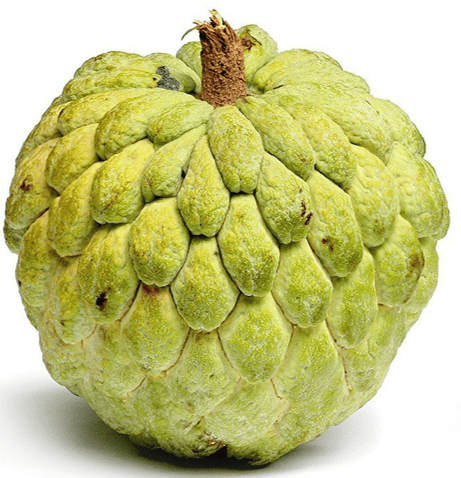
\includegraphics[width=0.8cm,height=0.8cm]{C8M11 - DT - Q3.png}} \adjustbox{scale=\scalefactor}{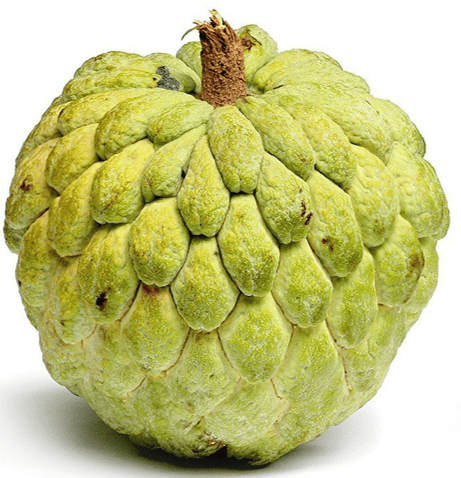
\includegraphics[width=0.8cm,height=0.8cm]{C8M11 - DT - Q3.png}} \adjustbox{scale=\scalefactor}{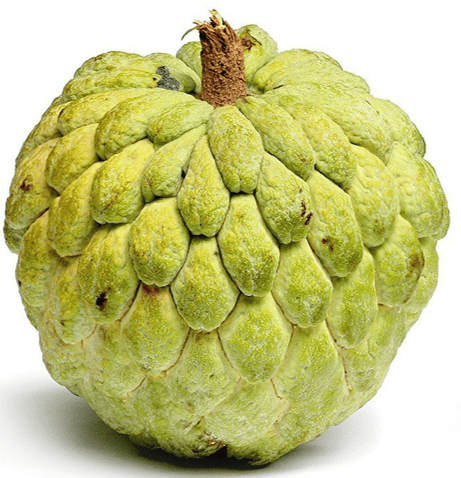
\includegraphics[width=0.8cm,height=0.8cm]{C8M11 - DT - Q3.png}} \adjustbox{scale=\scalefactor}{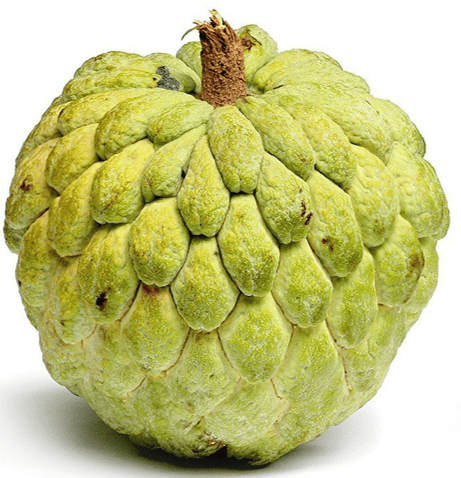
\includegraphics[width=0.8cm,height=0.8cm]{C8M11 - DT - Q3.png}} \adjustbox{scale=\scalefactor}{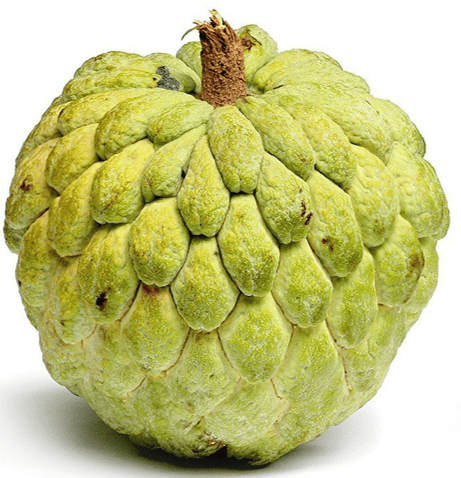
\includegraphics[width=0.8cm,height=0.8cm]{C8M11 - DT - Q3.png}} & Weight = 500 g \\
\hline
\adjustbox{scale=\scalefactor}{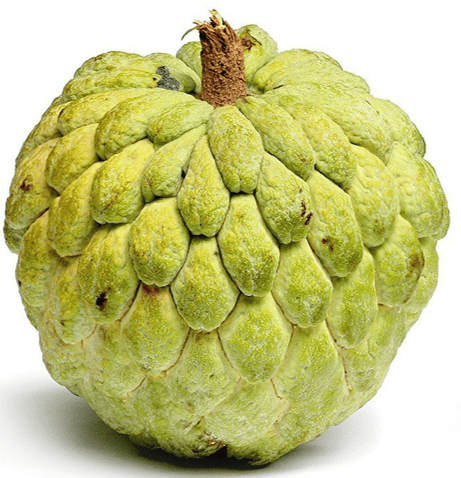
\includegraphics[width=0.8cm,height=0.8cm]{C8M11 - DT - Q3.png}} \adjustbox{scale=\scalefactor}{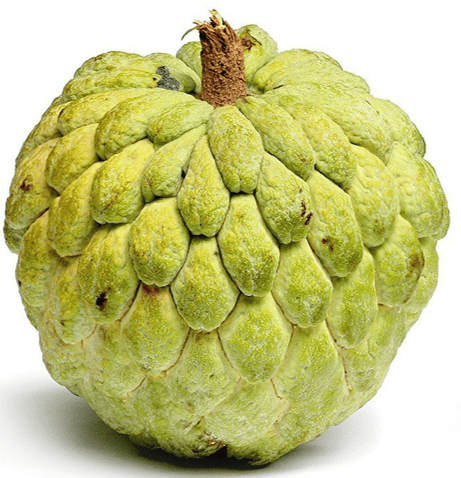
\includegraphics[width=0.8cm,height=0.8cm]{C8M11 - DT - Q3.png}} \adjustbox{scale=\scalefactor}{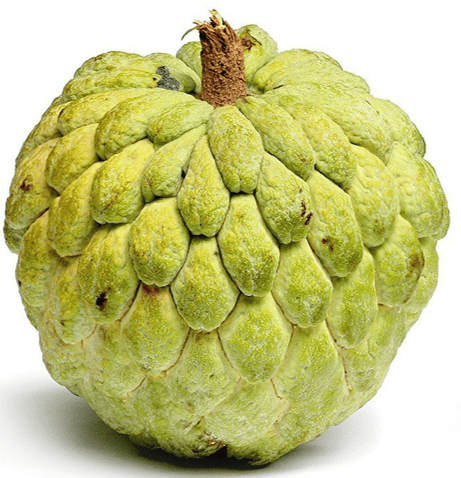
\includegraphics[width=0.8cm,height=0.8cm]{C8M11 - DT - Q3.png}} \adjustbox{scale=\scalefactor}{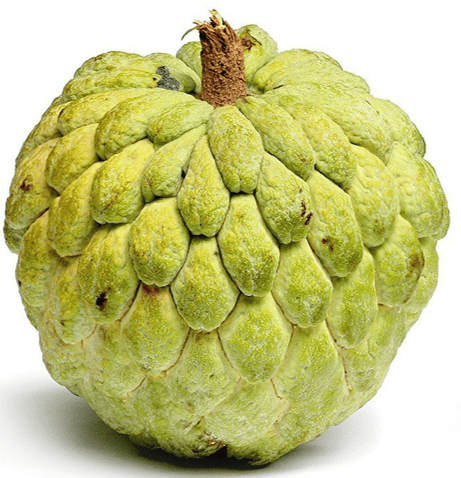
\includegraphics[width=0.8cm,height=0.8cm]{C8M11 - DT - Q3.png}} \adjustbox{scale=\scalefactor}{\includegraphics[width=0.8cm,height=0.8cm]{C8M11 - DT - Q3.png}} \adjustbox{scale=\scalefactor}{\includegraphics[width=0.8cm,height=0.8cm]{C8M11 - DT - Q3.png}} \adjustbox{scale=\scalefactor}{\includegraphics[width=0.8cm,height=0.8cm]{C8M11 - DT - Q3.png}} \adjustbox{scale=\scalefactor}{\includegraphics[width=0.8cm,height=0.8cm]{C8M11 - DT - Q3.png}} \adjustbox{scale=\scalefactor}{\includegraphics[width=0.8cm,height=0.8cm]{C8M11 - DT - Q3.png}} \adjustbox{scale=\scalefactor}{\includegraphics[width=0.8cm,height=0.8cm]{C8M11 - DT - Q3.png}} & Weight = \rule{40pt}{0.5pt} g\\
\hline
\end{tabular} },
optionA={10 g},
optionB={5 g},
optionC={1000 g},
optionD={500 g},
correctoption={C},
leftmini={0.7},
rightmini={0.15},
}

\begin{minipage}{\linewidth}
\hspace{1cm}
\centering
\tiny
\renewcommand{\arraystretch}{1.25}
\begin{tabular}{|M{1.2cm}|M{0.8cm}|M{0.8cm}|M{0.8cm}|M{0.8cm}|M{0.8cm}|}
\hline
Option & A (\ding{55}) & B (\ding{55}) & \cellcolor{cellgreen} C (\ding{51}) & D (\ding{55}) & E \\ 
\hline
8 A & \highno{0\%} & \highno{0\%} & \highgreen{92\%} & \highno{8\%} & \highno{0\%} \\ 
 \hline 
8 B & \highno{0\%} & \highno{0\%} & \highno{73\%} & \highno{27\%} & \highno{0\%} \\ \hline
\end{tabular}
\end{minipage}

\end{frame}
% \input{4. PPT/6. My Answer/Math/C8/117_C8M - Q27}


\begin{frame}[shrink=0.1,label=QPC8QC8M09 - DT - Q8]{Q18 [12. Factorization]}
\vspace{-0.2cm}
\mcqtextbottomOneFour{
questionnumber={18}, 
questionTag={C8M09 - DT - Q8}, 
questiontext={Identify the equation where the expression in the left-hand side is equal to the right-hand side.},
optionA={$2(2+z)$ = $4+z$},
optionB={$\frac{m+10}{10}$ = $m+1$},
optionC={$(x+y)^2 = x^2+y^2$},
optionD={$(10x)^2 = 100x^2$},
correctoption={D},
}

\begin{minipage}{\linewidth}
\hspace{1cm}
\centering
\tiny
\renewcommand{\arraystretch}{1.25}
\begin{tabular}{|M{1.2cm}|M{0.8cm}|M{0.8cm}|M{0.8cm}|M{0.8cm}|M{0.8cm}|}
\hline
Option & A (\ding{55}) & B (\ding{55}) & C (\ding{55}) & \cellcolor{cellgreen} D (\ding{51}) & E \\ 
\hline
8 A & \highno{31\%} & \highno{8\%} & \highno{38\%} & \highred{15\%} & \highno{8\%} \\ 
 \hline 
8 B & \highno{0\%} & \highno{13\%} & \highno{27\%} & \highno{60\%} & \highno{0\%} \\ \hline
\end{tabular}
\end{minipage}

\end{frame}
% \input{4. PPT/6. My Answer/Math/C8/117_C8M - Q18}


\begin{frame}[shrink=0.1,label=QPC8QC8M09 - DT - Q4]{Q23 [12. Factorization]}
\vspace{-0.2cm}
\mcqtextbottomOneFour{
questionnumber={23}, 
questionTag={C8M09 - DT - Q4}, 
questiontext={The expression $x^2+4x-21$ is in the form of \rule{50pt}{0.5pt}.},
optionA={$x^2+(a-b)x+ab$},
optionB={$x^2+(a+b)x+ab$},
optionC={$x^2+ax+ab$},
optionD={$by(ax-1)$},
correctoption={B},
}

\begin{minipage}{\linewidth}
\hspace{1cm}
\centering
\tiny
\renewcommand{\arraystretch}{1.25}
\begin{tabular}{|M{1.2cm}|M{0.8cm}|M{0.8cm}|M{0.8cm}|M{0.8cm}|M{0.8cm}|}
\hline
Option & A (\ding{55}) & \cellcolor{cellgreen} B (\ding{51}) & C (\ding{55}) & D (\ding{55}) & E \\ 
\hline
8 A & \highno{23\%} & \highred{8\%} & \highno{46\%} & \highno{15\%} & \highno{8\%} \\ 
 \hline 
8 B & \highno{53\%} & \highno{47\%} & \highno{0\%} & \highno{0\%} & \highno{0\%} \\ \hline
\end{tabular}
\end{minipage}

\end{frame}
% \input{4. PPT/6. My Answer/Math/C8/117_C8M - Q23}


\begin{frame}[shrink=0.1,label=QPC8QC8M09 - DT - Q7]{Q31 [12. Factorization]}
\vspace{-0.2cm}
\mcqtextbottomOneFour{
questionnumber={31}, 
questionTag={C8M09 - DT - Q7}, 
questiontext={Arjun bought $2z(7z-3)$ chocolates for rupees $112z^4 - 48z^3$. Help him find the price of each chocolate.},
optionA={Rs. $12z^2$},
optionB={Rs. $15z-4$},
optionC={Rs. $8z^2$},
optionD={Rs. $-22z-20$},
correctoption={C},
}

\begin{minipage}{\linewidth}
\hspace{1cm}
\centering
\tiny
\renewcommand{\arraystretch}{1.25}
\begin{tabular}{|M{1.2cm}|M{0.8cm}|M{0.8cm}|M{0.8cm}|M{0.8cm}|M{0.8cm}|}
\hline
Option & A (\ding{55}) & B (\ding{55}) & \cellcolor{cellgreen} C (\ding{51}) & D (\ding{55}) & E \\ 
\hline
8 A & \highno{15\%} & \highno{23\%} & \highred{23\%} & \highno{23\%} & \highno{15\%} \\ 
 \hline 
8 B & \highno{0\%} & \highno{20\%} & \highno{60\%} & \highno{7\%} & \highno{13\%} \\ \hline
\end{tabular}
\end{minipage}

\end{frame}
% \input{4. PPT/6. My Answer/Math/C8/117_C8M - Q31}


\begin{frame}[shrink=0.1,label=QPC8QC8M09 - DT - Q1]{Q45 [12. Factorization]}
\vspace{-0.2cm}
\mcqimgleftFourOne{
questionnumber={45}, 
questionTag={C8M09 - DT - Q1},
questiontext={Find the factors of the number of ice creams. },
imgtabletikz = { {\adjustbox{scale=\scalefactor}{\includegraphics[width=3cm,height=3cm]{C8M09 - DT - Q1.png}}} },
optionA={1, 2, 6},
optionB={4, 8, 12},
optionC={4, 40, 400},
optionD={1, 2, 4},
correctoption={D},
leftmini={0.5},
rightmini={0.4},
}

\begin{minipage}{\linewidth}
\hspace{1cm}
\centering
\tiny
\renewcommand{\arraystretch}{1.25}
\begin{tabular}{|M{1.2cm}|M{0.8cm}|M{0.8cm}|M{0.8cm}|M{0.8cm}|M{0.8cm}|}
\hline
Option & A (\ding{55}) & B (\ding{55}) & C (\ding{55}) & \cellcolor{cellgreen} D (\ding{51}) & E \\ 
\hline
8 A & \highno{8\%} & \highno{15\%} & \highno{23\%} & \highred{38\%} & \highno{15\%} \\ 
 \hline 
8 B & \highno{7\%} & \highno{13\%} & \highno{7\%} & \highno{60\%} & \highno{13\%} \\ \hline
\end{tabular}
\end{minipage}

\end{frame}
% \input{4. PPT/6. My Answer/Math/C8/117_C8M - Q45}


\begin{frame}[shrink=0.1,label=QPC8QC8M09 - DT - Q2]{Q56 [12. Factorization]}
\vspace{-0.2cm}
\mcqtextbottomOneFour{
questionnumber={56}, 
questionTag={C8M09 - DT - Q2}, 
questiontext={Find the common factor of 48$x^2y - 6xy$.},
optionA={6$xy$},
optionB={6$xy(8x - 1)$},
optionC={6$xy(8x + 1)$},
optionD={6$xy(x - 1)$},
correctoption={A},
}

\begin{minipage}{\linewidth}
\hspace{1cm}
\centering
\tiny
\renewcommand{\arraystretch}{1.25}
\begin{tabular}{|M{1.2cm}|M{0.8cm}|M{0.8cm}|M{0.8cm}|M{0.8cm}|M{0.8cm}|}
\hline
Option & \cellcolor{cellgreen} A (\ding{51}) & B (\ding{55}) & C (\ding{55}) & D (\ding{55}) & E \\ 
\hline
8 A & \highred{15\%} & \highno{77\%} & \highno{0\%} & \highno{8\%} & \highno{0\%} \\ 
 \hline 
8 B & \highno{40\%} & \highno{53\%} & \highno{0\%} & \highno{7\%} & \highno{0\%} \\ \hline
\end{tabular}
\end{minipage}

\end{frame}
% \input{4. PPT/6. My Answer/Math/C8/117_C8M - Q56}


\begin{frame}[shrink=0.1,label=QPC8QC8M19 - DT - Q5]{Q12 [13. Introduction to Graphs]}
\vspace{-0.2cm}
\mcqimgleftFourOne{
questionnumber={12}, 
questionTag={C8M19 - DT - Q5}, 
questiontext={From the given months, find the lowest sales percentage of Company A.},
imgtabletikz = { {\adjustbox{scale=\scalefactor}{\includegraphics[width=9cm,height=6cm]{C8M19 - DT - Q5i.png}}} }, 
optionA={60\%},
optionB={50\% },
optionC={80\%},
optionD={100\%},
correctoption={A},
leftmini={0.65},
rightmini={0.35},
}

\begin{minipage}{\linewidth}
\hspace{1cm}
\centering
\tiny
\renewcommand{\arraystretch}{1.25}
\begin{tabular}{|M{1.2cm}|M{0.8cm}|M{0.8cm}|M{0.8cm}|M{0.8cm}|M{0.8cm}|}
\hline
Option & \cellcolor{cellgreen} A (\ding{51}) & B (\ding{55}) & C (\ding{55}) & D (\ding{55}) & E \\ 
\hline
8 A & \highno{54\%} & \highno{15\%} & \highno{15\%} & \highno{8\%} & \highno{8\%} \\ 
 \hline 
8 B & \highgreen{87\%} & \highno{7\%} & \highno{7\%} & \highno{0\%} & \highno{0\%} \\ \hline
\end{tabular}
\end{minipage}

\end{frame}
% \input{4. PPT/6. My Answer/Math/C8/117_C8M - Q12}


\begin{frame}[shrink=0.1,label=QPC8QC8M19 - DT - Q7]{Q29 [13. Introduction to Graphs]}
\vspace{-0.2cm}
\mcqimgleftFourOne{
questionnumber={29}, 
questionTag={C8M19 - DT - Q7}, 
questiontext={Using the graph, how many paragraphs can we read in 14 hours?},
imgtabletikz = { {\adjustbox{scale=\scalefactor}{\includegraphics[width=9cm,height=6cm]{C8M19 - DT - Q7i.png}}} },
optionA={6},
optionB={3 },
optionC={3.5},
optionD={5.5},
correctoption={C},
leftmini={0.5},
rightmini={0.4},
}

\begin{minipage}{\linewidth}
\hspace{1cm}
\centering
\tiny
\renewcommand{\arraystretch}{1.25}
\begin{tabular}{|M{1.2cm}|M{0.8cm}|M{0.8cm}|M{0.8cm}|M{0.8cm}|M{0.8cm}|}
\hline
Option & A (\ding{55}) & B (\ding{55}) & \cellcolor{cellgreen} C (\ding{51}) & D (\ding{55}) & E \\ 
\hline
8 A & \highno{8\%} & \highno{23\%} & \highno{62\%} & \highno{8\%} & \highno{0\%} \\ 
 \hline 
8 B & \highno{0\%} & \highno{13\%} & \highgreen{87\%} & \highno{0\%} & \highno{0\%} \\ \hline
\end{tabular}
\end{minipage}

\end{frame}
% \input{4. PPT/6. My Answer/Math/C8/117_C8M - Q29}


\begin{frame}[shrink=0.1,label=QPC8QC8M19 - DT - Q3]{Q57 [13. Introduction to Graphs]}
\vspace{-0.2cm}
\mcqtextbottomOneFour{
questionnumber={57}, 
questionTag={C8M19 - DT - Q3}, 
questiontext={The coordinates of the origin are \rule{80pt}{0.5pt}.},
optionA={0 },
optionB={0,1 },
optionC={0, 0},
optionD={1, 1},
correctoption={C},
}

\begin{minipage}{\linewidth}
\hspace{1cm}
\centering
\tiny
\renewcommand{\arraystretch}{1.25}
\begin{tabular}{|M{1.2cm}|M{0.8cm}|M{0.8cm}|M{0.8cm}|M{0.8cm}|M{0.8cm}|}
\hline
Option & A (\ding{55}) & B (\ding{55}) & \cellcolor{cellgreen} C (\ding{51}) & D (\ding{55}) & E \\ 
\hline
8 A & \highno{23\%} & \highno{31\%} & \highred{23\%} & \highno{15\%} & \highno{8\%} \\ 
 \hline 
8 B & \highno{0\%} & \highno{33\%} & \highno{53\%} & \highno{13\%} & \highno{0\%} \\ \hline
\end{tabular}
\end{minipage}

\end{frame}
% \input{4. PPT/6. My Answer/Math/C8/117_C8M - Q57}

%

    